% ======================================================================
%  Unified constraint framework for exotic spin-dependent interactions
%  APS / REVTeX 4.2 manuscript, targeted at Physical Review D
%
%  Compile:  pdflatex main && pdflatex main
%  Figures are read from ../main_figures/ (see \graphicspath below); no
%  figure file is duplicated into this directory.
%
%  For a double-spaced single-column referee copy, replace the class
%  option "reprint" with "preprint".
% ======================================================================
\documentclass[
  aps,
  prd,
  reprint,
  amsmath,
  amssymb,
  nofootinbib,
  superscriptaddress,
  floatfix
]{revtex4-2}

\usepackage{graphicx}
\usepackage{bm}
\usepackage{booktabs}
\usepackage{array}
\usepackage{dcolumn}
\usepackage{hyperref}
\hypersetup{colorlinks=true,linkcolor=blue,citecolor=blue,urlcolor=blue}

\graphicspath{%
  {../main_figures/constraint_atlas/}%
  {../main_figures/gap_analysis/}%
  {../main_figures/matter_antimatter/}%
}

\newcommand{\Aalpha}{A_\alpha}
\newcommand{\sig}{\bm{\sigma}}

\begin{document}

\title{Unified constraint framework for exotic spin-dependent
interactions: a matter--antimatter sector comparison}

\author{Oyewo Temidayo Solomon}
\email{oyewodayo@gmail.com}
\affiliation{Department of Physics, Faculty of Science,
University of Ibadan, Ibadan, Nigeria}

\author{O.~E. Oyewande}
\affiliation{Department of Physics, Faculty of Science,
University of Ibadan, Ibadan, Nigeria}

\date{\today}

\begin{abstract}
Exotic spin-dependent interactions mediated by light, weakly coupled
bosons are described in two disjoint languages: the Standard Model
Extension (SME), a relativistic effective field theory of Lorentz and CPT
violation, and the Dobrescu--Mocioiu (DM) classification, a complete basis
of sixteen non-relativistic potentials $V_1$--$V_{16}$ in which
experiments report their bounds. We construct a systematic dictionary
between the two by applying the Foldy--Wouthuysen transformation to the SME
fermion-sector coefficients $b_\mu$, $d_{\mu\nu}$, $g_{\lambda\mu\nu}$ and
$H_{\mu\nu}$, and matching the resulting non-relativistic Hamiltonians onto
the DM basis. These four are shown to be the complete set generating
spin-dependent non-relativistic potentials: $a_\mu$, $c_{\mu\nu}$ and
$e_\mu$ appear only in spin-independent terms and $f_\mu$ not at all
through third order in $1/m$, so none has an image in the DM basis. All
four reductions are obtained in full and agree with the literature,
including the
momentum-linear $d_{ij}$ and $d_{00}$ components, whose apparent sign
discrepancy we trace to a momentum-index convention in the reference
result rather than to the derivation. We then define a
dimensionless CPT asymmetry parameter
$\Aalpha=(g_\alpha^{f}-g_\alpha^{\bar f})/(g_\alpha^{f}+g_\alpha^{\bar
f})$ and evaluate it against a compiled database of 283 experimental
constraint datasets, 247 of which enter the analysis, standardized to a
common interaction-range axis.
Fifteen matter--antimatter pairs can be compared, and all exhibit
statistically significant asymmetry after correction for autocorrelation
among interpolated points. We show analytically, and confirm across all
fifteen pairs, that $\Aalpha$ constructed from one-sided experimental upper
bounds cannot by itself distinguish CPT violation from an ordinary
sensitivity gap between the two experiments. A spin-independent scalar
channel in our sample shows an asymmetry comparable to the spin-dependent
ones. The
binding constraint on this class of CPT test is therefore the absence of
antimatter-sector measurements rather than statistical power. Only 22 of
247 analyzed datasets involve an antimatter sector, and seven of twelve
classified potentials have none at all. A coverage analysis identifies the
$e$-$N$, $n$-$N$ and $p$-$N$ sectors and the $V_{1a}$, $V_{9+10}$ and
$V_{12+13}$ potentials as the largest opportunities for new measurement.
The mapping table, database and analysis pipeline are released as an
extensible resource.
\end{abstract}

\maketitle

% ======================================================================
\section{Introduction}
\label{sec:intro}

The Standard Model is tested to extraordinary precision yet remains
incomplete: it does not accommodate quantum gravity, offers no dark matter
candidate, and does not explain the observed baryon asymmetry
\cite{Planck2018}. A well-motivated class of extensions introduces light,
weakly coupled bosonic fields, such as axions, axion-like particles and
dark photons, that mediate feeble long-range forces, a possibility first set
out systematically by Moody and Wilczek \cite{MoodyWilczek1984}. Those that couple to
fermion spin rather than to charge or mass alone are of particular
interest, since spin has no classical analogue and therefore offers an
unusually clean channel for probing symmetry violation.

Two formalisms describe such interactions, and they are not directly
commensurable. The SME of Colladay and Kostelecký
\cite{Colladay1997,Colladay1998}, motivated by the spontaneous Lorentz
breaking identified in string theory \cite{KosteleckySamuel1989}, is a
relativistic effective field theory
that parametrizes Lorentz and CPT violation through fixed background
coefficients such as $b_\mu$, $H_{\mu\nu}$ and $d_{\mu\nu}$; its
coefficients are catalogued and constrained in the data tables of
Kostelecký and Russell \cite{KosteleckyRussell2011}. The DM
classification \cite{Dobrescu2006} is a complete non-relativistic basis of
sixteen potentials $V_1$--$V_{16}$, generated by single-boson exchange
between two fermions and recast in coordinate space for laboratory use in
Ref.~\cite{Fadeev2019}, in which essentially all laboratory searches
report their limits; experiments up to 2024 are reviewed in
Ref.~\cite{Cong2025}. Translating between the two
requires the Foldy--Wouthuysen (FW) transformation \cite{Foldy1950}, the
standard technique for extracting the non-relativistic limit of a
relativistic Dirac Hamiltonian.

Separately, antimatter precision physics has become one of the sharpest
available probes of fundamental symmetry. Experiments at CERN compare
matter and antimatter magnetic moments and spectral lines at a level that
directly tests CPT invariance \cite{Smorra2017,Ahmadi2017}. Joining these
two threads suggests a concrete observable: a CPT-violating
spin-dependent interaction should appear as an asymmetry between the
coupling constants inferred for matter and for antimatter.

No complete dictionary between the SME and DM bases has been published,
and no framework exists for using such a dictionary to compare
matter-sector and antimatter-sector constraints within a single
quantitative measure. Prior mappings are partial, restricted to subsets of
coefficients or potentials, and the constraint literature itself is
reported in inconsistent units and conventions, which obstructs direct
comparison across platforms. This paper supplies both the dictionary and
the comparison framework, and reports what the currently published data
can establish and what they cannot.

Section~\ref{sec:mapping} presents the FW reductions, establishes which
coefficients can contribute at all, and gives the resulting SME$\to$DM
matching table. Section~\ref{sec:asymmetry} defines the
asymmetry parameter and derives the central interpretive limitation on it.
Section~\ref{sec:methods} describes the compiled database and the
statistical methodology. Sections~\ref{sec:results} and \ref{sec:gaps}
report the matched-pair results and the coverage analysis.
Section~\ref{sec:limitations} states the limitations of the present
database, and Sec.~\ref{sec:conclusions} concludes.

% ======================================================================
\section{SME-to-DM mapping}
\label{sec:mapping}

\subsection{The \texorpdfstring{$b_\mu$}{b-mu} coefficient}
\label{sec:bmu}

The CPT-odd term $\mathcal{L}_b=-b_\mu\bar\psi\gamma_5\gamma^\mu\psi$
separates into a spatial part $b_i$, which is even and therefore exact at
order $m^0$, and a temporal part $b_0$, which is odd and enters only at
order $1/m$. In the Dirac representation
$\gamma^0\gamma_5\gamma^i=-\Sigma^i$, so projected onto the upper block
\begin{equation}
  H_{\rm NR}(b_i) = -\mathbf{b}\cdot\sig \qquad (\text{matter}),
  \label{eq:bi-matter}
\end{equation}
already in non-relativistic form with no further FW iteration required.
The temporal component is odd, since
$\gamma^0\gamma_5\gamma^0=-\gamma_5$, and so contributes through the FW
cross-term between the free odd operator $\bm{\alpha}\cdot\mathbf{p}$ and
the perturbing odd operator $\mathcal{O}_{b_0}=-b_0\gamma_5$. Retaining
only the piece linear in $b_0$,
\begin{equation}
  H_{\rm NR}(b_0)
  = \frac{\beta}{2m}\{\bm{\alpha}\cdot\mathbf{p},\mathcal{O}_{b_0}\}
    \Big|_{\rm upper}
  = -\frac{b_0(\sig\cdot\mathbf{p})}{m} + O(m^{-2}).
\end{equation}

The antiparticle sector follows from the lower block by the hole-theory
reinterpretation. An antiparticle of momentum $\mathbf p$ and spin
$\mathbf s$ is the absence of a negative-energy solution of momentum
$-\mathbf p$ and spin $-\mathbf s$, with the opposite energy. A CPT test
compares a particle with its CPT-conjugate state, an antiparticle of the
same momentum and reversed spin. Labelling that state by the particle's
spin operator gives
\begin{equation}
  H^{\bar f}_{\rm NR}(\mathbf p,\sig) = -H_{\rm lower}(-\mathbf p,\sig).
  \label{eq:anti-rule}
\end{equation}
Since $\Sigma^i={\rm diag}(\sigma^i,\sigma^i)$ repeats the \emph{same}
operator in the upper ($\beta=+1$) and lower ($\beta=-1$) blocks,
\begin{equation}
  \langle{\rm u}|b_i\gamma^0\gamma_5\gamma^i|{\rm u}\rangle
  = \langle{\rm l}|b_i\gamma^0\gamma_5\gamma^i|{\rm l}\rangle
  = -b_i\sigma^i ,
  \label{eq:bi-block}
\end{equation}
and since $b_i$ carries no momentum,
\begin{equation}
  H^{\bar f}_{\rm NR}(b_i)
  = -\left(-\mathbf{b}\cdot\sig\right) = +\mathbf{b}\cdot\sig .
  \label{eq:bi-anti}
\end{equation}

The CPT-conjugate antiparticle receives the opposite shift. This
matter--antimatter sign flip is the signature of a CPT-odd coefficient. It is \emph{not} a charge-conjugation effect on the
axial-vector bilinear $\bar\psi\gamma_5\gamma^\mu\psi$, which is $C$-even
for every $\mu$ and therefore cannot by itself produce the difference
between Eqs.~\eqref{eq:bi-matter} and \eqref{eq:bi-anti}. The difference is
a CPT effect and appears only when CPT-conjugate states are compared.

Stated at fixed physical spin, the result looks different. An antiparticle
with the particle's spin has energy $-\mathbf b\cdot\mathbf s$, the same
as the particle. This is Kostelecký and Lane's antiparticle rule, which
leaves $b_\mu$, $c_{\mu\nu}$ and $g_{\lambda\mu\nu}$ unchanged and reverses
$a_\mu$, $d_{\mu\nu}$, $e_\mu$, $f_\mu$ and $H_{\mu\nu}$
\cite{KosteleckyLane1999b}. The two statements are equivalent, since a
spin-linear term changes sign when the spin is reversed. The CPT-conjugate
comparison is the one relevant to a CPT test: with it, exact CPT symmetry
gives $g^{\bar f}_\alpha=g^f_\alpha$. We verified both comparisons
symbolically for every coefficient family, using the full FW reduction and
kinetic-sector field redefinition. The CPT-conjugate comparison reproduces
each coefficient's CPT parity in every family, and the fixed-spin
comparison reproduces the rule of Ref.~\cite{KosteleckyLane1999b} in every
family. Both require the momentum reversal in Eq.~\eqref{eq:anti-rule};
omitting it changes the result for every term odd in $\mathbf p$. The
result also agrees with Bluhm, Kostelecký and Russell \cite{Bluhm1999}.
Their substitution rule from hydrogen to antihydrogen reverses $a_\mu$,
$d_{\mu\nu}$ and $H_{\mu\nu}$ but not $b_\mu$, the fixed-spin rule. Their
$b_\mu$-dependent 1S--2S shift nevertheless changes sign, because the
antihydrogen hyperfine states compared have opposite positron and
antiproton spin assignments, that is, CPT-conjugate spin states.

Promoting Eq.~\eqref{eq:bi-matter} to a two-body potential by pairing the
same vertex on both fermions gives the spin--spin structure
\begin{equation}
  V_2(r) = -g_A^{(1)}g_A^{(2)}\frac{1}{4\pi}
           (\sig_1\cdot\sig_2)\frac{e^{-r/\lambda}}{r},
  \label{eq:V2}
\end{equation}
identifying $b_i$ with $V_2$ at leading order, while $b_0$ matches the
velocity-dependent $V_8$ at order $1/m$.

\subsection{The \texorpdfstring{$H_{\mu\nu}$}{H-mu-nu} coefficient}

$H_{\mu\nu}$ is CPT-even but Lorentz-odd: CPT-conjugate matter and
antimatter states receive identical shifts at tree level, so its
experimental signature is a sidereal anisotropy rather than a
matter--antimatter asymmetry. Its magnetic-like
spatial components $H_{ij}$ are even and generate, at order $m^0$, using
$\gamma^0\sigma^{ij}|_{\rm upper}=\varepsilon^{ijk}\sigma^k$,
\begin{equation}
  H_{\rm NR}(H_{ij}) = +\bm{\mathcal{H}}_B\cdot\sig ,
  \qquad \mathcal{H}_B^k = \tfrac12\varepsilon^{ijk}H_{ij},
\end{equation}
matching the dipole--dipole potential $V_3$. The electric-like mixed
components $H_{0i}$ are odd, since $\gamma^0\sigma^{0i}=i\gamma^i$ is
block-off-diagonal, and generate at order $1/m$, through the same FW
cross-term used for $b_0$ with $\mathcal{O}_{H_E}=i\sum_k H_{0k}\gamma^k$,
\begin{equation}
  H_{\rm NR}(H_{0i})
  = +\frac{1}{m}\sig\cdot(\mathbf{p}\times\mathbf{H}_E),
  \qquad H_E^i \equiv H_{0i},
\end{equation}
matching the spin--velocity potential $V_7$. Applying
Eq.~\eqref{eq:anti-rule} gives $H^{\bar f}_{\rm NR}=H^{f}_{\rm NR}$ for
both components, as their CPT-even character requires; at fixed physical
spin the sign reverses, in line with the rule $H_{\mu\nu}\to-H_{\mu\nu}$
of Ref.~\cite{KosteleckyLane1999b}. This coefficient therefore gives
$g^{\bar f}_\alpha=g^f_\alpha$ and $\Aalpha=0$ for the underlying
couplings, in contrast to $b_\mu$.

\subsection{The \texorpdfstring{$d_{\mu\nu}$}{d-mu-nu} coefficient}

Following Kostelecký and Lane \cite{KosteleckyLane1999}, $d_{\mu\nu}$ is
a CPT-even, traceless, kinetic-sector coefficient entering through the
derivative coupling $\mathcal{L}_d=\tfrac12 i\bar\psi
d^{\mu\nu}\gamma_5\gamma_\mu\overleftrightarrow{\partial}_\nu\psi$. With
$\Gamma_\mu\equiv\gamma^0\gamma_5\gamma_\mu$ one finds $\Gamma_0=-\gamma_5$
(odd) and $\Gamma_i=+\Sigma^i$ (even), from which
\begin{align}
  H_{\rm NR}(d_{i0}) &= +d_{i0}\,m\,\sigma^i          &&\to V_2, \\
  H_{\rm NR}(d_{ij}) &= +d_{ij}\,p^j\sigma^i          &&\to V_7,V_8,\\
  H_{\rm NR}(d_{00}) &= +d_{00}(\sig\cdot\mathbf{p})  &&\to V_8 .
\end{align}
All three results reproduce the non-relativistic Hamiltonian of
Ref.~\cite{KosteleckyLane1999} exactly, including signs, once that
reference's momentum convention is applied. The convention is not stated
explicitly alongside their Eq.~(4), which describes $p_j$ as the
three-momentum of the particle, but it is fixed unambiguously by the
free-particle term of the same authors' intermediate relativistic
Hamiltonian \cite{KosteleckyLane1999b}, $m\mathcal{P}_0 :=
-p_j\gamma^0\gamma^j$. That expression equals $-\bm\alpha\cdot\mathbf p$,
so recovering the free Dirac Hamiltonian $+\bm\alpha\cdot\mathbf p+\beta m$
requires their lower-index $p_j$ to be the covariant component
$p_j=-p^j$. Read as the physical three-momentum instead, the two
momentum-linear terms appear to differ by an overall sign while the
mass-enhanced term still agrees. That pattern points to a momentum-index
mismatch, not a derivation error. We have verified the
correspondence symbolically, including an independent implementation of
the kinetic-sector field redefinition $A=1-\tfrac12\gamma^0(\Gamma_0-\gamma_0)$
of Ref.~\cite{KosteleckyLane1999b}.

\subsection{The \texorpdfstring{$g_{\lambda\mu\nu}$}{g-lambda-mu-nu} coefficient}
\label{sec:gmunu}

$g_{\lambda\mu\nu}$ is CPT-odd and dimensionless, and enters the
kinetic sector through $\tfrac12 g_{\lambda\mu\nu}\sigma^{\lambda\mu}$ in
$\Gamma_\nu$. It is antisymmetric in its first two indices, since
$\sigma^{\lambda\mu}$ is. Because it modifies $\Gamma_0$, the same field
redefinition used for $d_{\mu\nu}$ applies; we verified that the resulting
Hamiltonian is Hermitian before reducing it.

The reduction separates by index family. Writing
$\tilde g_j\equiv\tfrac12\varepsilon_{jkl}g_{kl0}$ for the dual of the
spatial--spatial, $\nu=0$ block, and $(\mathbf{g}_{00})_k\equiv g_{k00}$,
\begin{align}
  H_{\rm NR}(g_{[kl]0}) &= -\,m\,\tilde{\mathbf g}\cdot\sig  &&\to V_2, \\
  H_{\rm NR}(g_{[0k]0}) &= +\,\sig\cdot(\mathbf p\times\mathbf{g}_{00}) &&\to V_7, \\
  H_{\rm NR}(g_{[kl]j}) &= +\tfrac12\varepsilon_{klm}g_{mlj}\,p^j\,\sigma^k &&\to V_7,V_8 .
\end{align}
The remaining family $g_{[0k]j}$ gives no contribution at this order.

Applying Eq.~\eqref{eq:anti-rule} to each family gives an exact sign flip
for all three contributing families, as the CPT-odd character of
$g_{\lambda\mu\nu}$ requires. The momentum reversal is essential here: the
$g_{[0k]0}$ and $g_{[kl]j}$ terms are linear in $\mathbf p$, and comparing
the lower block at the same momentum instead would wrongly suggest that
these two families do not flip. At fixed physical spin, all three families
give identical particle and antiparticle shifts, in line with the rule
$g_{\lambda\mu\nu}\to+g_{\lambda\mu\nu}$ of Ref.~\cite{KosteleckyLane1999b}.
The matter--antimatter signature is therefore set by the coefficient's CPT
parity, for $g_{\lambda\mu\nu}$ as for $b_\mu$.

The three surviving structures reproduce those already obtained for the
other coefficients: the $\nu=0$ spatial--spatial block is Zeeman-like and
mass-enhanced, as $b_i$ and $d_{i0}$ are; the $\nu=0$
temporal--spatial block is the spin--velocity form found for $H_{0i}$; and
the $\nu=j$ spatial--spatial block has the general
$\tilde g_{kj}p^j\sigma^k$ shape found for $d_{ij}$. All three agree with
Ref.~\cite{KosteleckyLane1999} term by term, under the same covariant
momentum convention established in Sec.~\ref{sec:mapping} for
$d_{\mu\nu}$. Since that convention was fixed without reference to $g$,
this is an independent check on it.

\subsection{Coefficients that generate no spin-dependent terms}
\label{sec:nospin}

The four coefficients treated above exhaust the spin-dependent sector.
Splitting the non-relativistic Hamiltonian of Ref.~\cite{KosteleckyLane1999}
into its top-level terms, every term carrying a factor of $\sig$ contains
only $b_\mu$, $d_{\mu\nu}$, $g_{\lambda\mu\nu}$ and $H_{\mu\nu}$. The
coefficients $a_\mu$, $c_{\mu\nu}$ and $e_\mu$ appear exclusively in
spin-independent terms, and $f_\mu$ does not appear in the non-relativistic
Hamiltonian at all through third order in $1/m$.

This is why the dictionary presented here is complete rather than partial:
the Dobrescu--Mocioiu basis is spin-dependent apart from $V_1$, so the
excluded coefficients have no image in it at these orders. The
$g_sg_s\cdot V_1\cdot e$-$e^+$ pair of Sec.~\ref{sec:results} lies in
this spin-independent sector, which receives contributions from $a_\mu$,
$c_{\mu\nu}$ and $e_\mu$ but from none of the four coefficients above.

\subsection{Master matching table}

Table~\ref{tab:master} synthesizes the four reductions. Its final column
gives the relation between the particle and antiparticle couplings for
CPT-conjugate states. It describes the underlying couplings, not the
published bounds: as Sec.~\ref{sec:asymmetry} shows, an $\Aalpha$ built
from one-sided bounds cannot reveal it.

\begin{table*}[t]
\caption{\label{tab:master}%
Master SME$\to$DM matching table, covering the complete set of SME
coefficients that generate spin-dependent non-relativistic potentials
($b_\mu$, $d_{\mu\nu}$, $g_{\lambda\mu\nu}$, $H_{\mu\nu}$); see
Sec.~\ref{sec:nospin} for why the remainder are excluded. Here
$\tilde g_j\equiv\tfrac12\varepsilon_{jkl}g_{kl0}$ and
$(\mathbf g_{00})_k\equiv g_{k00}$.
The final column relates particle and antiparticle couplings for
CPT-conjugate states (antiparticle spin reversed), verified symbolically for
every row; it follows the coefficient's CPT parity without exception. At
fixed physical spin every sign in that column reverses
\cite{KosteleckyLane1999b}. Neither relation gives $|\Aalpha|\to1$: a flip
makes the signed $\Aalpha$ diverge [Eq.~\eqref{eq:divergence}] and equal
couplings give $\Aalpha=0$, so a value near unity in the data reflects a
sensitivity gap between independent bounds (Sec.~\ref{sec:asymmetry}).}
\begin{ruledtabular}
\begin{tabular}{llllll}
SME coeff. & CPT & Non-relativistic Hamiltonian & DM potential(s) &
$1/m$ order & Matter--antimatter \\
\colrule
$b_i$      & Odd  & $-\mathbf{b}\cdot\sig$ (matter); $+\mathbf{b}\cdot\sig$ (CPT-conj.\ antimatter) & $V_2$      & $m^{0}$        & $g^{\bar f}=-g^{f}$ \\
$b_0$      & Odd  & $-b_0(\sig\cdot\mathbf{p})/m$                                        & $V_8$      & $m^{-1}$       & $g^{\bar f}=-g^{f}$ \\
$H_{ij}$   & Even & $+\bm{\mathcal{H}}_B\cdot\sig$                                       & $V_3$      & $m^{0}$        & $g^{\bar f}=g^{f}$ \\
$H_{0i}$   & Even & $+\frac{1}{m}\sig\cdot(\mathbf{p}\times\mathbf{H}_E)$                & $V_7$      & $m^{-1}$       & $g^{\bar f}=g^{f}$ \\
$d_{i0}$   & Even & $+d_{i0}\,m\,\sigma^i$                                               & $V_2$      & $m^{+1}$       & $g^{\bar f}=g^{f}$ \\
$d_{ij}$   & Even & $+d_{ij}\,p^j\sigma^i$                                               & $V_7,V_8$  & $m^{0}$ (vel.) & $g^{\bar f}=g^{f}$ \\
$d_{00}$   & Even & $+d_{00}(\sig\cdot\mathbf{p})$                                       & $V_8$      & $m^{0}$ (mom.) & $g^{\bar f}=g^{f}$ \\
$g_{[kl]0}$& Odd  & $-m\,\tilde{\mathbf g}\cdot\sig$                                       & $V_2$      & $m^{+1}$       & $g^{\bar f}=-g^{f}$ \\
$g_{[0k]0}$& Odd  & $+\sig\cdot(\mathbf p\times\mathbf{g}_{00})$                           & $V_7$      & $m^{0}$        & $g^{\bar f}=-g^{f}$ \\
$g_{[kl]j}$& Odd  & $+\tfrac12\varepsilon_{klm}g_{mlj}p^j\sigma^k$                        & $V_7,V_8$  & $m^{0}$ (vel.) & $g^{\bar f}=-g^{f}$ \\
\end{tabular}
\end{ruledtabular}
\end{table*}

% ======================================================================
\section{The CPT asymmetry parameter}
\label{sec:asymmetry}

For a coupling $\alpha$ constrained independently in a matter sector and
its conjugate antimatter sector, we define the dimensionless asymmetry
\begin{equation}
  \Aalpha(\lambda)
  = \frac{g_\alpha^{f}(\lambda)-g_\alpha^{\bar f}(\lambda)}
         {g_\alpha^{f}(\lambda)+g_\alpha^{\bar f}(\lambda)},
  \label{eq:asymmetry}
\end{equation}
evaluated as a function of interaction range $\lambda$, where the
antifermion coupling refers to the CPT-conjugate state (same momentum,
reversed spin). With this definition, exact CPT invariance gives
$g^{\bar f}_\alpha=g^f_\alpha$ and hence $\Aalpha=0$.

It is tempting to substitute the signed relation $g_{\bar f}=-g_f$ implied
by Eqs.~\eqref{eq:bi-matter} and \eqref{eq:bi-anti} directly into
Eq.~\eqref{eq:asymmetry}. Doing so gives
\begin{equation}
  \Aalpha = \frac{g-(-g)}{g+(-g)} = \frac{2g}{0}\longrightarrow\infty,
  \label{eq:divergence}
\end{equation}
The ratio diverges (we confirmed this with a symbolic limit); it does not
approach unity.

This is not, however, the quantity that published data can supply. The
inputs $g_f$ and $g_{\bar f}$ are independent, strictly positive
experimental \emph{upper bounds}, not signed measurements of one
underlying coupling. For any two independent positive bounds $g_1,g_2$ the
ratio $(g_1-g_2)/(g_1+g_2)$ approaches $\pm1$ whenever one bound is far
tighter than the other, \emph{regardless of the underlying physics}:
setting $g_{\rm tight}=r\,g_{\rm loose}$ and taking $r\to0^+$ gives
$\Aalpha\to1$ with no CPT content at all.

Consequently an observed $|\Aalpha|\approx1$ is \emph{consistent with},
but is not \emph{evidence for}, a non-zero $b_\mu$: the same numerical
pattern is what independent bounds of very different sensitivity produce
even under exact CPT symmetry. This governs the interpretation of every
asymmetry reported below, and we treat it as one of the main results of
this work, not a side remark. Its practical consequence is that the most
informative pairs are those with the \emph{lowest} asymmetry, since those
are the pairs in which the two sectors are probed at comparable
sensitivity.

% ======================================================================
\section{Database and methods}
\label{sec:methods}

\subsection{Compilation and standardization}

We compiled 283 experimental constraint datasets from the published
literature, drawing on the compilation of Ref.~\cite{Cong2025} and the
underlying primary sources, spanning nitrogen-vacancy-center magnetometry
\cite{Rong2018a,Rong2018b,Jiao2020}, torsion balances
\cite{Hoskins1985,Kapner2007,Heckel2008,Tan2020,Lee2020}, atomic
co-magnetometers \cite{Vasilakis2009}, precision spectroscopy of simple
atoms and molecules
\cite{Alighanbari2020,Salumbides2014,Delaunay2017,Ficek2017}, Casimir-force
measurements \cite{Bordag2001,Chen2016}, and antimatter and exotic-atom
spectroscopy, including positronium and antiprotonic helium
\cite{Adkins2022,Ficek2018,Fadeev2022}. Each dataset is a digitized exclusion curve $g(\lambda)$ or
$\alpha(\lambda)$.

Datasets are parsed for coupling family, DM potential label, fermion
sector, and source. A bare numeric prefix in the source filenames denotes
the potential number itself, so a \texttt{3}-prefixed file bounds $V_3$
alone and only a \texttt{23} prefix denotes the $V_2+V_3$ combination.
Every potential assignment was validated against the source compilation's
own curation records; among the 194 datasets those records cover there is
no disagreement. Interaction ranges reported variously in meters,
MeV$^{-1}$, eV$^{-1}$, centimeters, nanometers and femtometers are
converted to a common meter scale by a unit-detection routine applied
before any downstream analysis. Bounds published as a gravity-normalized
Yukawa strength $|\alpha|$ are kept separate from those published as a
coupling $|g|$; typical values of the two differ by more than thirty
orders of magnitude.

\subsection{Exclusions}

Of the 283 compiled datasets, 36 are held out of the analysis, leaving
247. Twenty-eight are combined envelope curves, twelve in $g_Ag_V$ and
sixteen in $g_pg_s$, that aggregate several experiments; the source compilation assigns them no
single potential and flags them for review, and no single $V_n$ applies to
an envelope by construction. One is an astrophysical $e$-$N$ bound with no
potential assignment that can be established from the source. Two are
contributor-template placeholders. Five are the 90\% confidence-level
variants of the Cong \textit{et al.} hydrogen bounds \cite{Cong2025b},
which the source ships alongside the 95\% CL curves; they are the same
measurement at a second confidence level, so retaining both would
double-count the experiment. Every exclusion is recorded
individually with a stated reason, and the registry retains all 283 rows
so that the compiled and analyzed counts remain separately auditable.

\subsection{Pairing and statistics}

Two datasets are matched into a matter--antimatter pair only when they
share coupling family, DM potential label and interaction class, their
fermion sectors are physically conjugate (for example $ee$ with
$e\bar{e}$), and exactly one is flagged as antimatter. This logic is
conservative: it will not match datasets differing in
potential classification even where their sectors are conjugate.

For each matched pair both curves are interpolated log-linearly in
$\log\lambda$--$\log g$ onto a common log-spaced grid of 300 points
spanning the overlapping $\lambda$ range, and $\Aalpha(\lambda)$ is
evaluated at every point. Significance is assessed in four stages, each
addressing a limitation of the previous one:

\begin{enumerate}
\item A uniform $\chi^2$ test assuming a flat 10\% fractional uncertainty
      at every grid point.
\item A weighted $\chi^2$ test estimating a per-point fractional
      uncertainty from the local curvature of each curve in log--log
      space, on the grounds that a smoothly varying published bound is
      better determined than one with sharp local features.
\item Both tests above treat the 300 grid points as independent, which is
      unjustified: they are interpolated from far fewer real measurements
      along smooth curves, so adjacent points are strongly correlated. An
      effective number of degrees of freedom is estimated from the
      autocorrelation length $\tau$ of the $\chi^2$ residuals in
      grid-index space (the lag at which the residual autocorrelation first
      falls below $1/e$), as $n_{\rm eff}=n/\tau$. The weighted $\chi^2$ is
      scaled down by the same factor, $\chi^2_{\rm eff}=\chi^2\,n_{\rm
      eff}/n$, and compared with a $\chi^2$ distribution on $n_{\rm eff}$
      degrees of freedom. Most of the resulting $p$-values lie far below
      double precision, so we quote the equivalent one-sided Gaussian
      significance $Z$.
\item A parametric bootstrap (2000 resamples) gives a 95\% confidence
      interval on the mean $|\Aalpha|$. Each resample perturbs both
      interpolated couplings by their estimated fractional uncertainties
      (log-normally, so they stay positive) and recomputes $\Aalpha$
      exactly.
\end{enumerate}

Two points about the bootstrap matter for how its intervals are read.
Because $|\Aalpha|$ is nonlinear in the couplings, folded at zero and
saturating at one, the resampled means sit slightly off the point estimate
even when the perturbations are symmetric. We remove that offset, estimated
as the median bootstrap bias, before quoting the interval. And the interval
only reflects the spread implied by the assumed curve uncertainties; for
$|\Aalpha|$ an interval that excludes zero is not, on its own, evidence of a
non-zero asymmetry.

All analysis is performed by \textsc{Spindep}, an open, version-controlled
pipeline; the full analysis is reproducible from a single command, and the
parsing, matching and statistical modules are covered by an automated test
suite.

% ======================================================================
\section{Results}
\label{sec:results}

\subsection{The compiled database}

The 247 analyzed datasets divide by coupling family as $g_Ag_A$ (66),
$g_sg_s$ (49), $g_Vg_V$ (44), $g_pg_s$ (37), $g_Ag_V$ (25), $g_pg_p$ (15)
and an unlabeled $V_1$ family (11). By DM potential the database is
dominated by $V_{4+5}$ (61), followed by $V_1$ (47), $V_3$ (39),
$V_{9+10}$ (31), $V_2$ (20) and $V_{12+13}$ (16), with $V_{1a}$ (14),
$V_{11}$ (7), $V_8$ (6), $V_{2+3}$ (2), $V_{16}$ (2) and $V_{15}$ (2)
making up the remainder. Several labels combine adjacent catalogue potentials that the
underlying experiments do not distinguish; $V_6$, $V_7$ and $V_{14}$ have
no classified dataset at all. Figure~\ref{fig:atlas} shows the constraint
atlas for $V_3$, the best-covered potential in the antimatter sector.

Only 22 of the 247 analyzed datasets involve an antimatter sector: 9 in
$e$-$\bar p$, 6 in $e$-$\bar\mu$ (muonium), 5 in $e$-$e^+$, and one each
in $\bar p$-He and the $dd\mu^+$ molecular ion. Muonium bounds are counted
on the antimatter side because the atom contains an antimuon, the same
reason $dd\mu^+$ is. This imbalance, 22 antimatter datasets against 225
matter-sector ones, is the central empirical fact of this work.

\begin{figure*}[t]
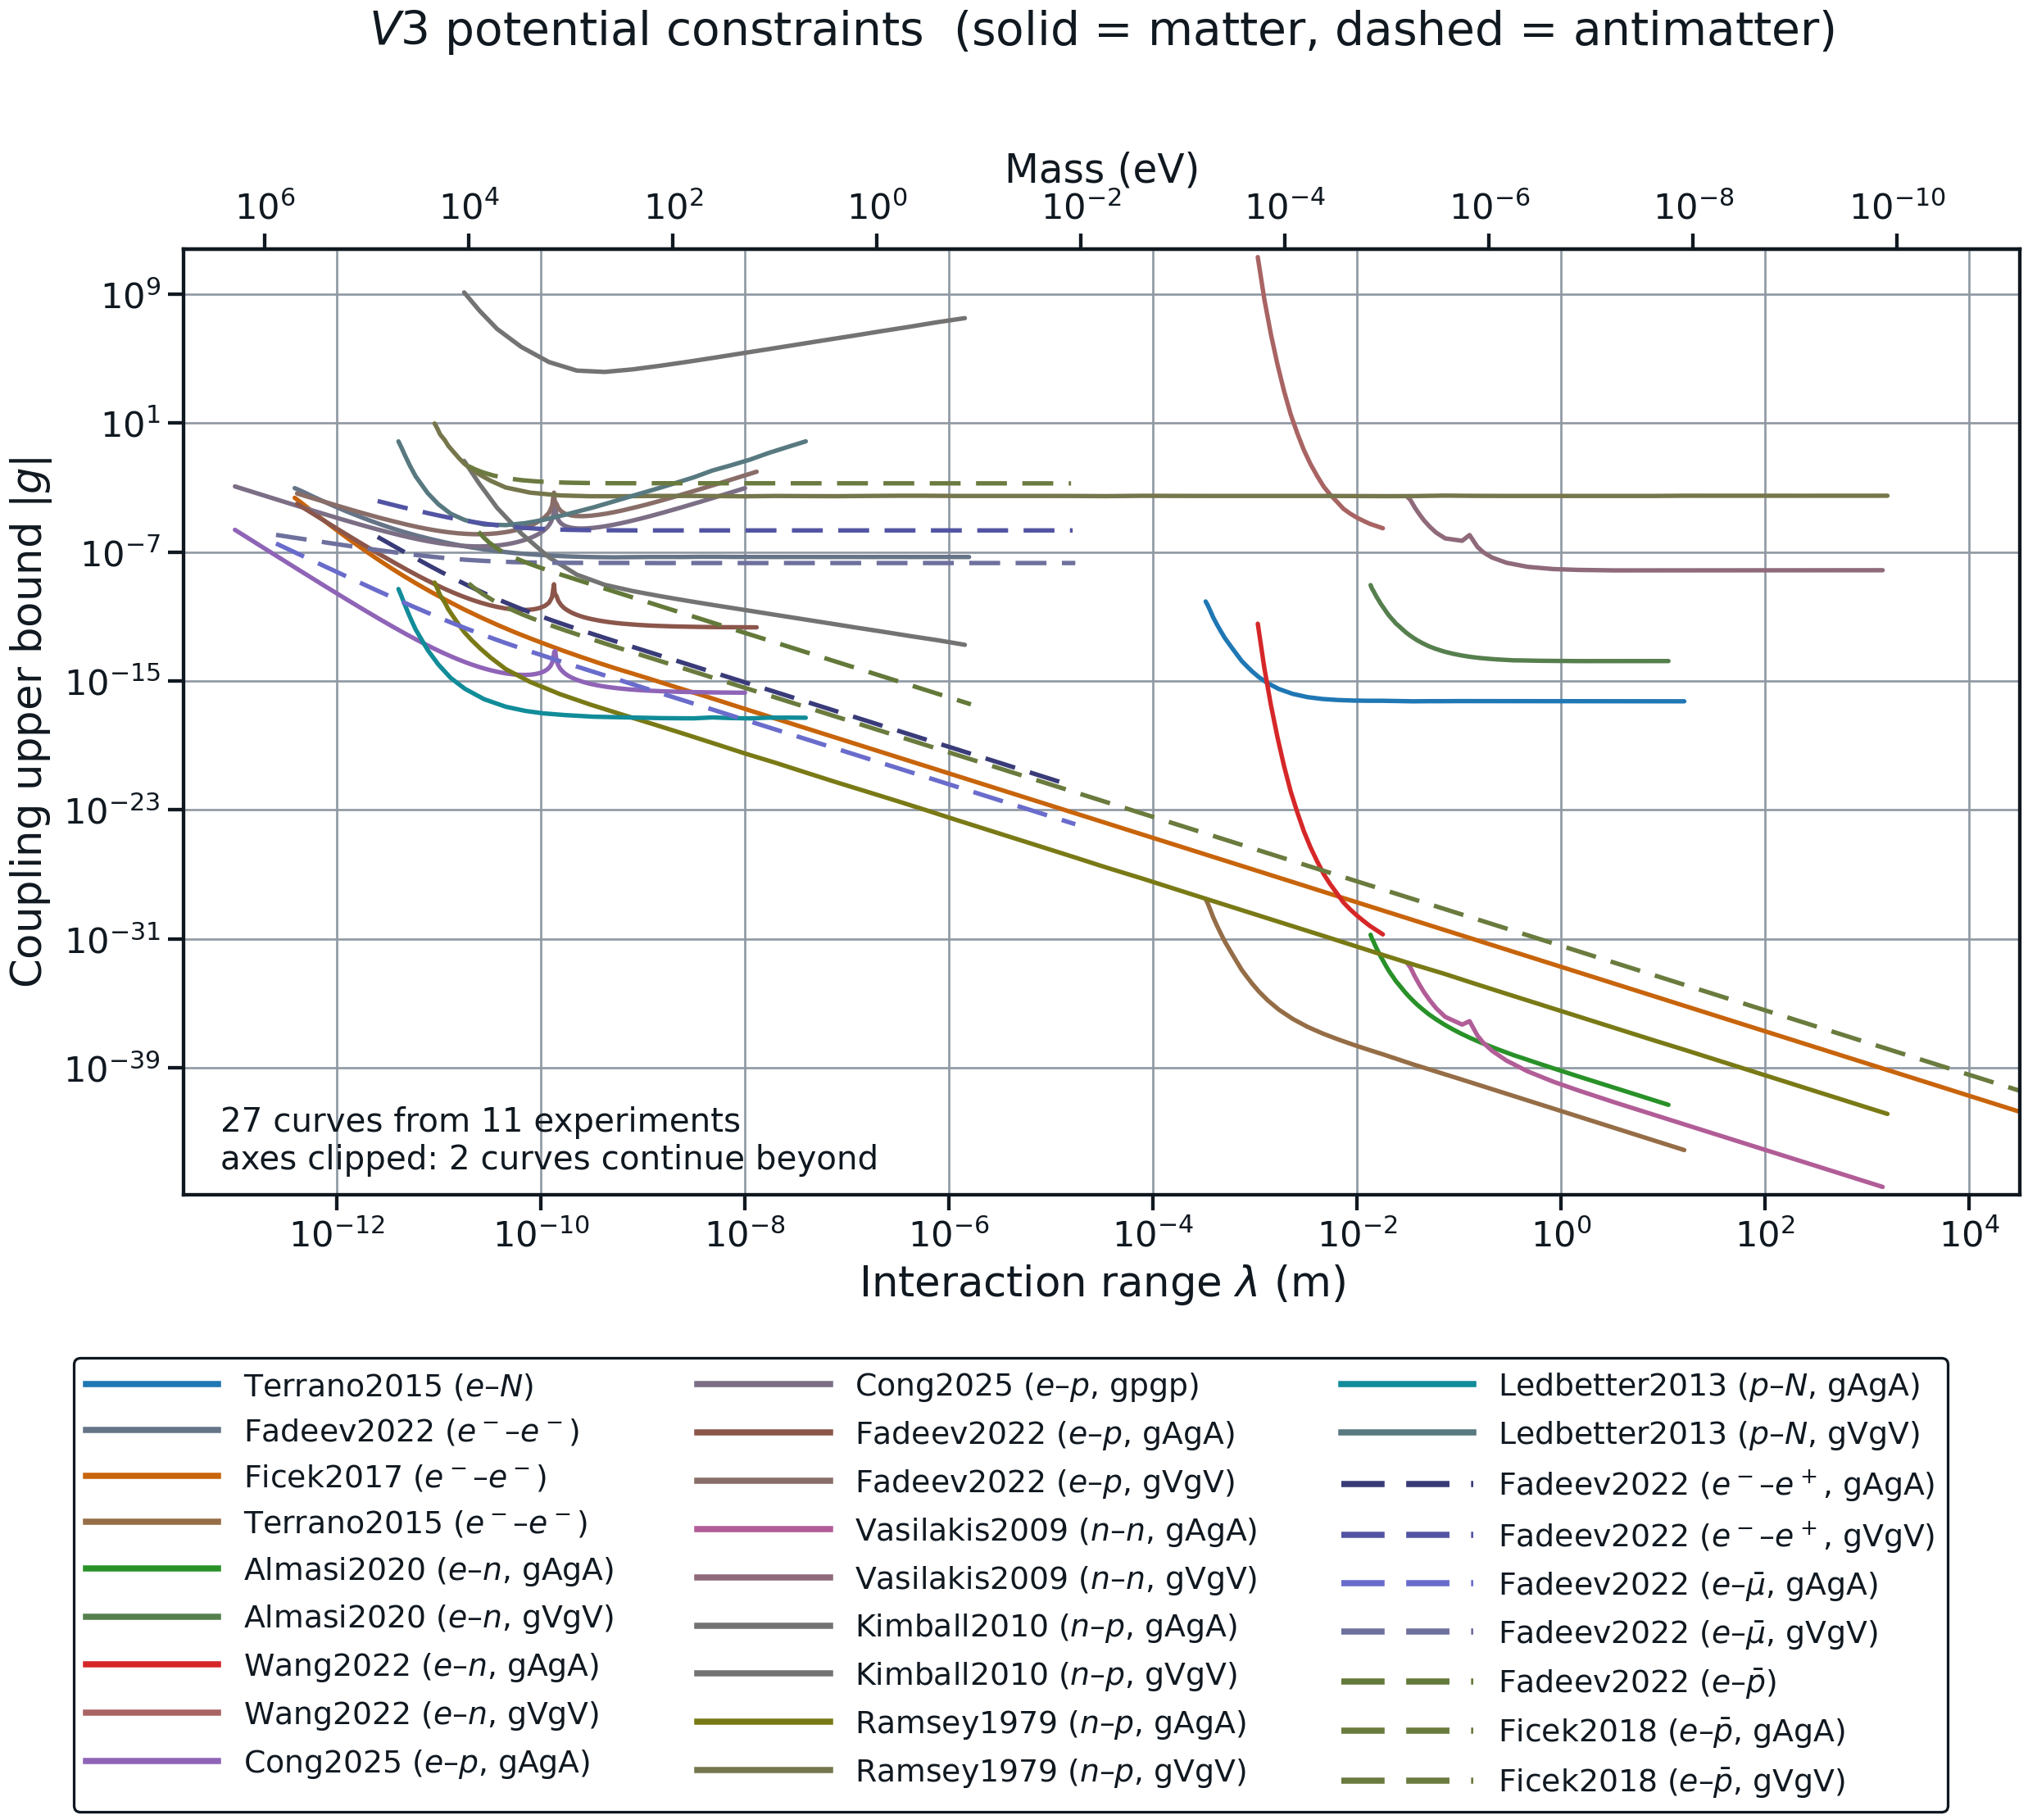
\includegraphics[width=0.92\textwidth]{constraint_V3.png}
\caption{\label{fig:atlas}%
Constraint atlas for $V_3$, the potential with the broadest
antimatter-sector coverage in the compiled database. Solid curves are
matter-sector bounds, dashed curves antimatter-sector; the region above
each curve is excluded. Shown at full page width because the panel
carries 27 curves from 11 experiments.}
\end{figure*}

\subsection{Matched pairs}

The pairing logic returns fifteen matter--antimatter pairs, listed in
Table~\ref{tab:pairs} with the mean absolute asymmetry, the
autocorrelation-corrected effective degrees of freedom, the resulting
significance, and the 95\% bootstrap interval.

Effective degrees of freedom range from 6 to 21 across the fifteen pairs, a
factor of 14--50 below the 300 grid points, so the correction is far from
cosmetic. Every pair stays significant after it. The weakest is the
Jiao/Karshenboim $e$-$e^+$ pair at $Z=5.1$ ($p\approx2\times10^{-7}$); the
others lie between $Z=26$ and $Z=51$.

Two rows repeat two others. The source compilation files the same Fadeev
\textit{et al.}\ $V_3$ curves under both $g_Vg_V$ and $g_pg_p$, so the
$g_Vg_V$ and $g_pg_p$ pairs built from them give identical numbers. The
fifteen pairs therefore contain thirteen independent comparisons.

\begin{table*}[t]
\caption{\label{tab:pairs}%
All fifteen matched matter--antimatter pairs, with the
autocorrelation-corrected effective degrees of freedom
$\mathrm{dof}_{\rm eff}$, the weighted-$\chi^2$ significance $Z$ after that
correction, and the 95\% bootstrap confidence interval on the mean
asymmetry. Per Sec.~\ref{sec:asymmetry}, a value near unity is consistent
with, but not evidence for, CPT violation.}
\begin{ruledtabular}
\begin{tabular}{lllldccl}
Coupling & Potential & Sector & Matter / antimatter source &
\multicolumn{1}{c}{$\overline{|\Aalpha|}$} & $\mathrm{dof}_{\rm eff}$ &
$Z$ & 95\% CI \\
\colrule
$g_Ag_A$ & $V_3$ & $e$-$\bar p$ & Cong \cite{Cong2025b} / Fadeev \cite{Fadeev2022} & 1.0000 & 8 & 51.1 & [1.0000, 1.0000] \\
$g_Ag_A$ & $V_2$ & $e$-$\bar p$ & Cong \cite{Cong2025b} / Ficek \cite{Ficek2018} & 0.9999 & 21 & 34.4 & [0.9999, 0.9999] \\
$g_Ag_A$ & $V_2$ & $e$-$\bar p$ & Karshenboim \cite{Karshenboim2011} / Ficek \cite{Ficek2018} & 0.9998 & 17 & 38.8 & [0.9998, 0.9998] \\
$g_Ag_A$ & $V_2$ & $e$-$e^+$ & Ficek \cite{Ficek2017} / Karshenboim \cite{Karshenboim2011} & 0.9892 & 21 & 48.2 & [0.9886, 0.9896] \\
$g_Ag_A$ & $V_3$ & $e$-$e^+$ & Ficek \cite{Ficek2017} / Fadeev \cite{Fadeev2022} & 0.9539 & 6 & 38.5 & [0.9518, 0.9557] \\
$g_Vg_V$ & $V_3$ & $e$-$e^+$ & Fadeev \cite{Fadeev2022} / Fadeev \cite{Fadeev2022} & 0.9535 & 6 & 37.1 & [0.9516, 0.9552] \\
$g_pg_p$ & $V_3$ & $e$-$e^+$ & Fadeev \cite{Fadeev2022} / Fadeev \cite{Fadeev2022} & 0.9535 & 6 & 37.1 & [0.9516, 0.9552] \\
$g_pg_p$ & $V_3$ & $e$-$\bar p$ & Cong \cite{Cong2025b} / Ficek \cite{Ficek2018} & 0.9304 & 6 & 34.3 & [0.9293, 0.9314] \\
$g_Ag_A$ & $V_3$ & $e$-$\bar p$ & Cong \cite{Cong2025b} / Ficek \cite{Ficek2018} & 0.9303 & 6 & 34.3 & [0.9292, 0.9313] \\
$g_sg_s$ & $V_1$ & $e$-$e^+$ & Delaunay \cite{Delaunay2017} / Adkins \cite{Adkins2022} & 0.8727 & 21 & 25.7 & [0.8686, 0.8770] \\
$g_Ag_A$ & $V_3$ & $e$-$\bar p$ & Fadeev \cite{Fadeev2022} / Ficek \cite{Ficek2018} & 0.8236 & 6 & 37.3 & [0.8168, 0.8299] \\
$g_Ag_A$ & $V_3$ & $e$-$\bar p$ & Fadeev \cite{Fadeev2022} / Fadeev \cite{Fadeev2022} & 0.8044 & 8 & 43.8 & [0.8024, 0.8063] \\
$g_Vg_V$ & $V_3$ & $e$-$\bar p$ & Fadeev \cite{Fadeev2022} / Ficek \cite{Ficek2018} & 0.7994 & 7 & 31.8 & [0.7971, 0.8015] \\
$g_pg_p$ & $V_3$ & $e$-$\bar p$ & Fadeev \cite{Fadeev2022} / Ficek \cite{Ficek2018} & 0.7994 & 7 & 31.8 & [0.7971, 0.8015] \\
$g_Ag_A$ & $V_2$ & $e$-$e^+$ & Jiao \cite{Jiao2020} / Karshenboim \cite{Karshenboim2011} & 0.3336 & 9 & 5.1 & [0.3197, 0.3474] \\
\end{tabular}
\end{ruledtabular}
\end{table*}

\subsection{Interpretation}

By Sec.~\ref{sec:asymmetry}, an asymmetry near unity in
Table~\ref{tab:pairs} is consistent with, but not evidence for, CPT
violation: a large sensitivity gap between the two measurements produces
the same signature regardless of the underlying physics. This applies to
every row, including the three $e$-$\bar p$ pairs at 0.9998 and above at the
top of the table.

The $g_sg_s\cdot V_1\cdot e$-$e^+$ pair at 0.8727 makes the same point
from a different direction. $V_1$ is spin-independent, so none of the
coefficients in Table~\ref{tab:master} feeds it, yet its asymmetry sits
well inside the range spanned by the $g_Ag_A$ pairs (0.33 to 1.00). A high asymmetry is simply what two
bounds of very different sensitivity produce, whatever channel they sit in. Figures~\ref{fig:highest} and \ref{fig:lowest} contrast the
highest- and lowest-asymmetry pairs.

The lowest entry, 0.3336 for the $g_Ag_A\cdot V_2\cdot e$-$e^+$ pair of Refs.~\cite{Jiao2020,Karshenboim2011},
is the pair whose two bounds are closest in sensitivity, and is therefore the
single most informative datum currently available for constraining $b_\mu$
in the $e$-$e^+$ channel, because it is not saturated.

The four pairs built on the recent hydrogen-spectroscopy bounds of
Ref.~\cite{Cong2025b} show the effect directly. Each can be set against a
pair with the same coupling, potential and antimatter partner but an older
$e$-$p$ bound on the matter side, and in all four the newer bound gives the
higher asymmetry: 0.9999 against 0.9998 for $g_Ag_A\cdot V_2$ with
Ficek \textit{et al.}, 1.0000 against 0.8044 for $g_Ag_A\cdot V_3$ with
Fadeev \textit{et al.}, and 0.9303 against 0.8236 ($g_Ag_A$) and 0.9304
against 0.7994 ($g_pg_p$) for $V_3$ with Ficek \textit{et al.} Improving
the matter-sector measurement, with no change to the antimatter sector and
none to the underlying physics, drove the asymmetry \emph{up}. This is a direct empirical confirmation of
the argument of Sec.~\ref{sec:asymmetry}: $\Aalpha$ built from one-sided
bounds tracks the sensitivity ratio, not CPT status.

\begin{figure}[t]
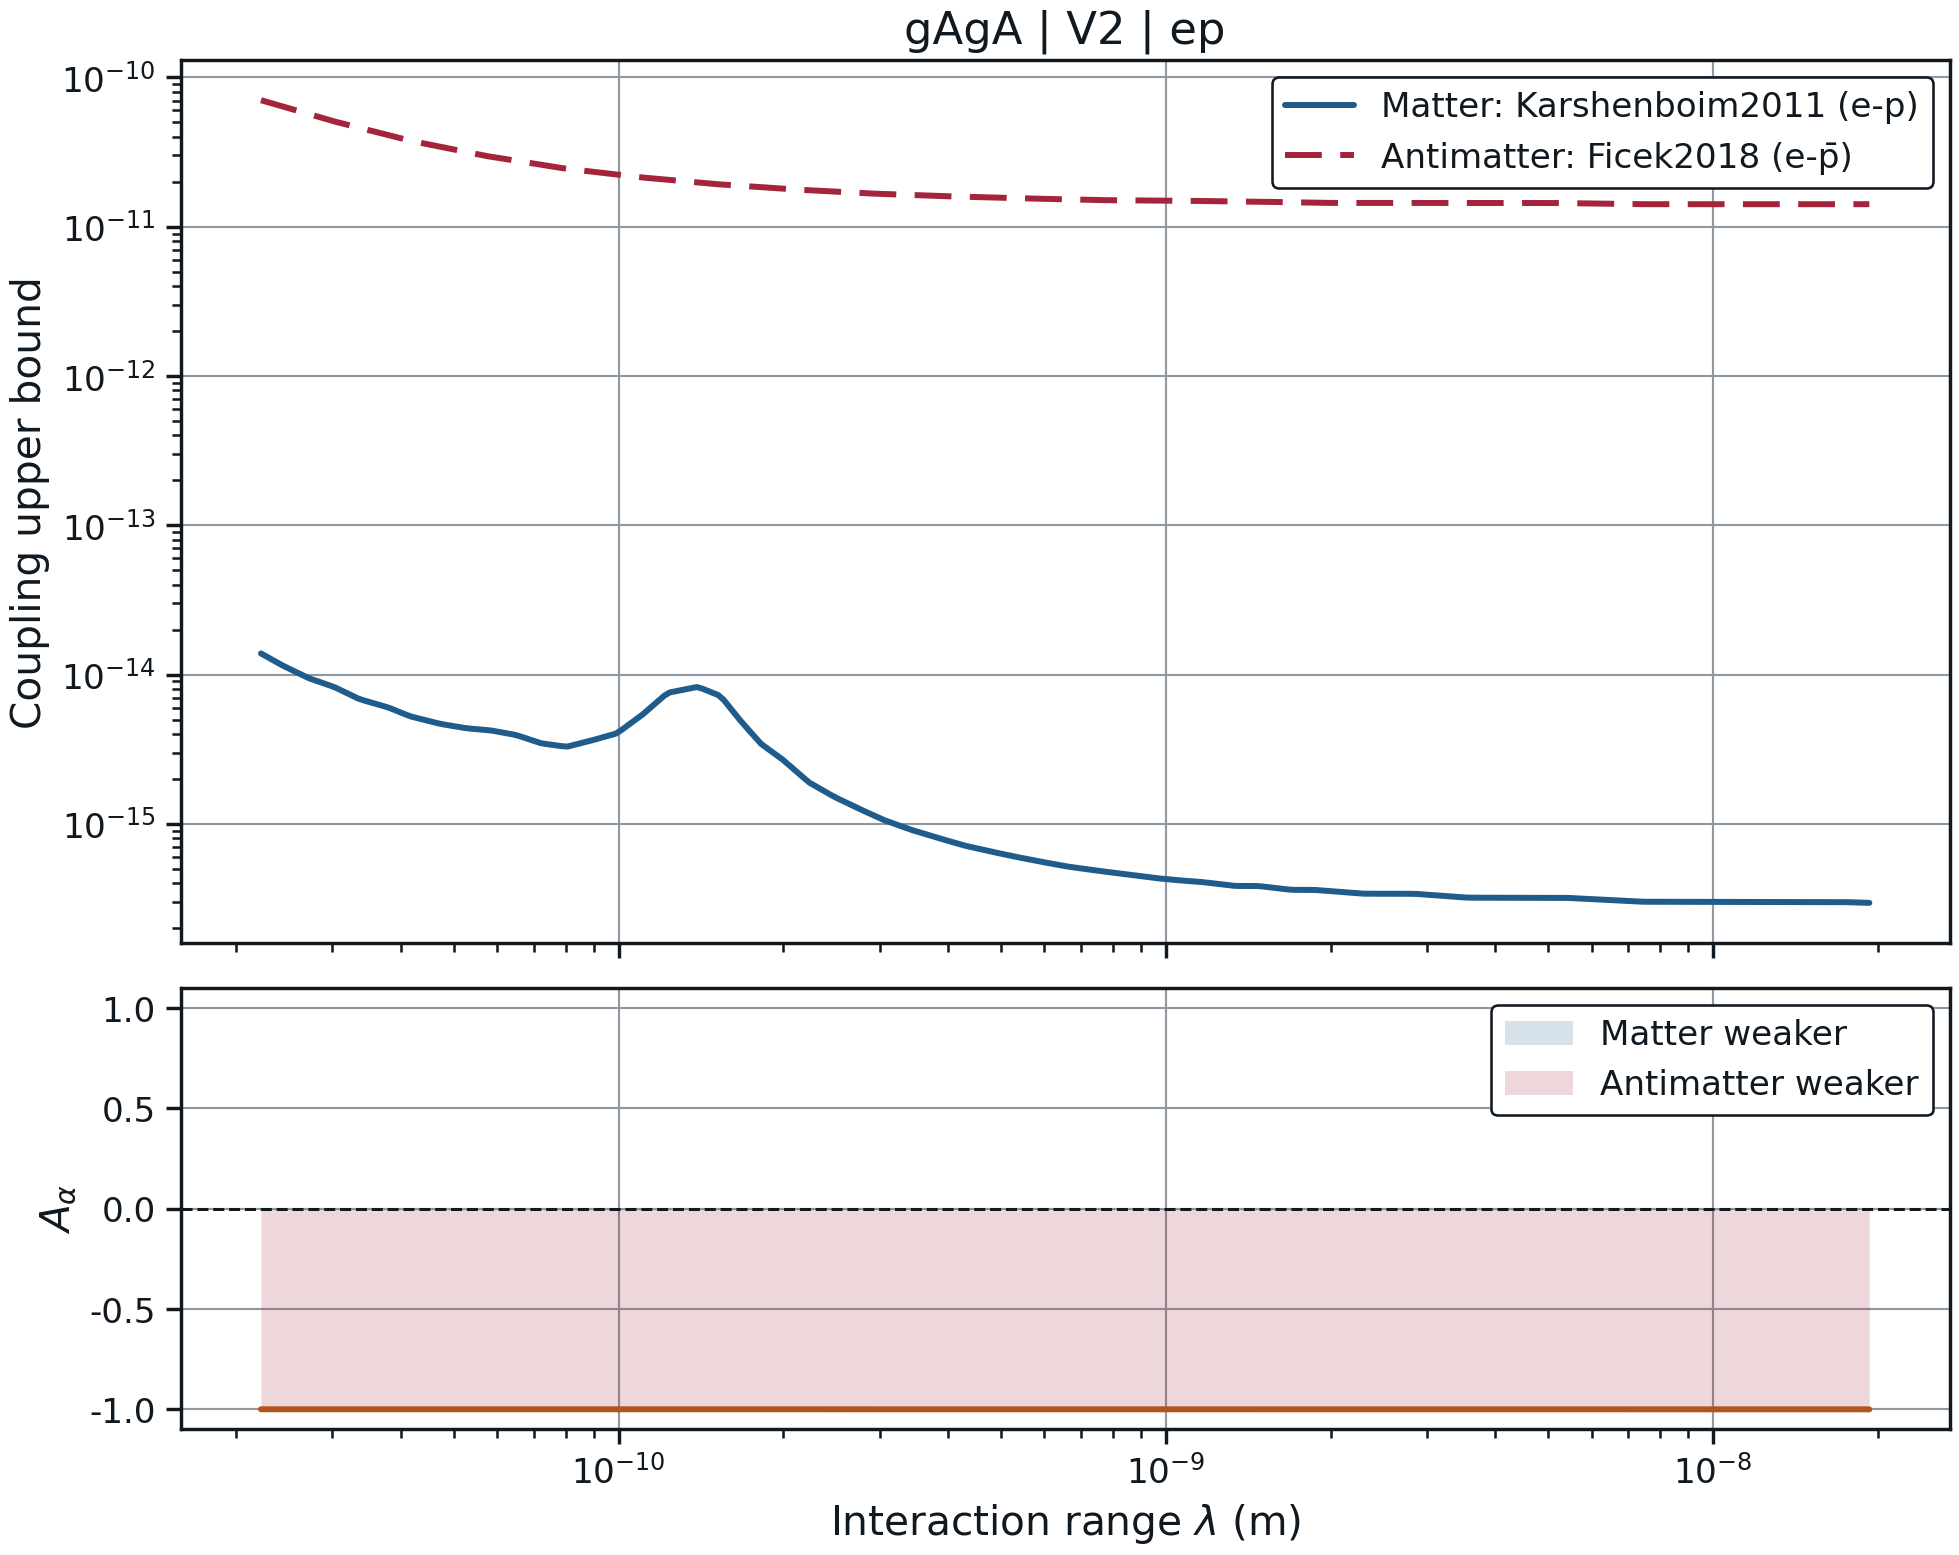
\includegraphics[width=\columnwidth]{gAgA_V2_ep_Karshenboim2011_vs_Ficek2018.png}
\caption{\label{fig:highest}%
Matter--antimatter comparison for the $g_Ag_A\cdot V_2\cdot e$-$\bar p$
pair of Refs.~\cite{Karshenboim2011,Ficek2018}, one of the three highest
asymmetries in the database ($\overline{|\Aalpha|}=0.9998$). The two bounds differ by orders of
magnitude in sensitivity over the overlapping range, which is sufficient
on its own to saturate $\Aalpha$.}
\end{figure}

\begin{figure}[t]
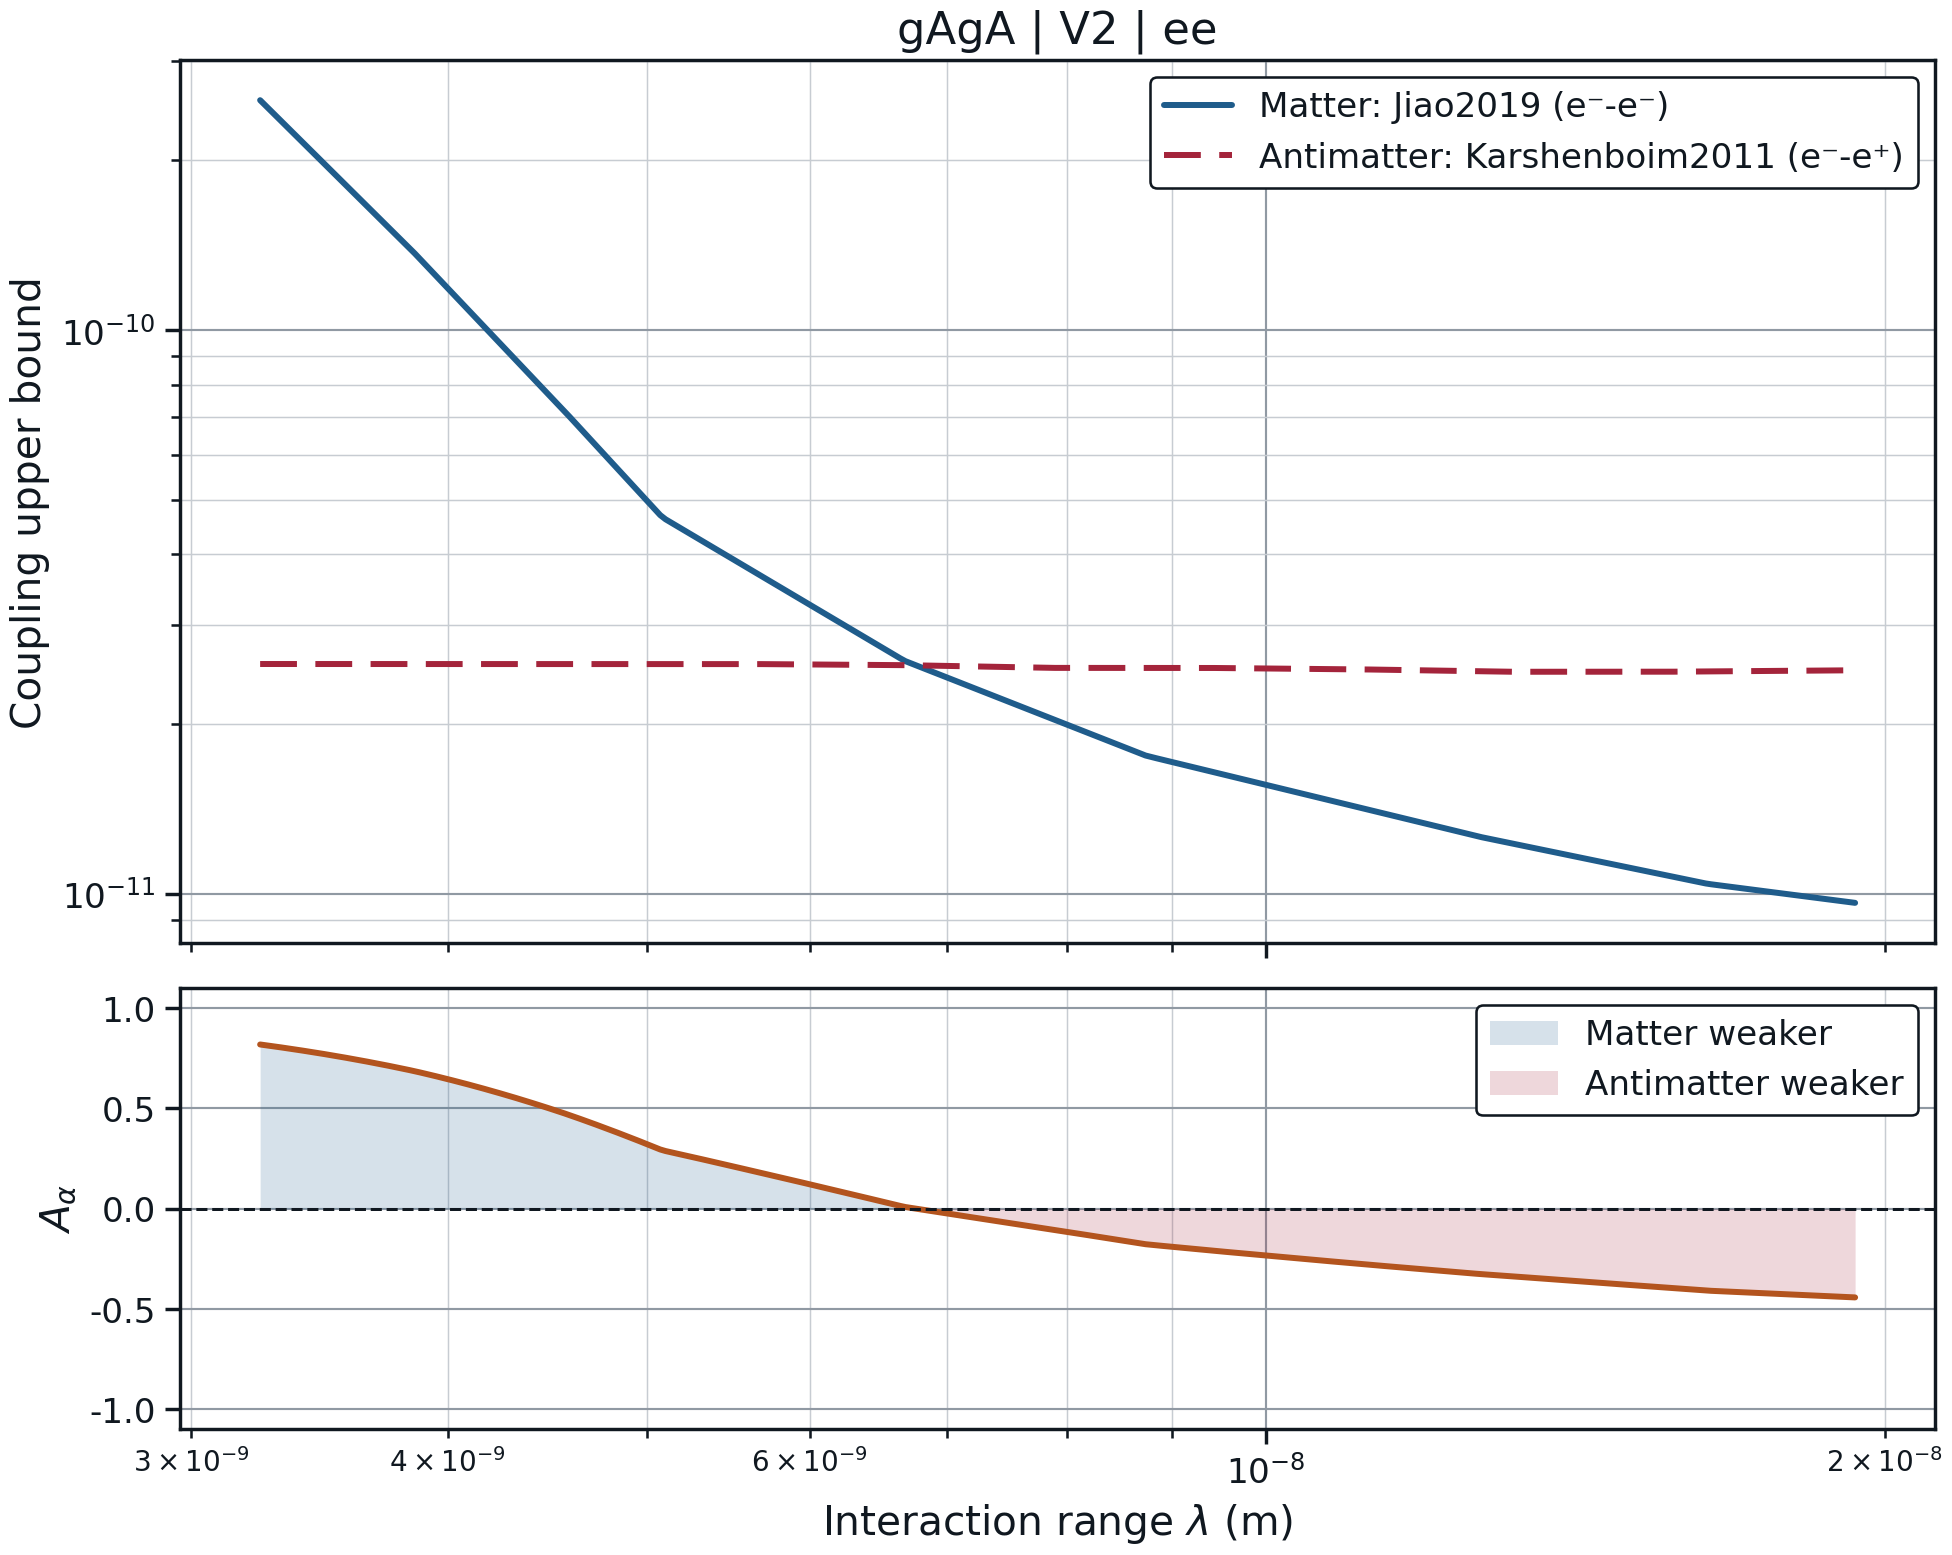
\includegraphics[width=\columnwidth]{gAgA_V2_ee_Jiao2019_vs_Karshenboim2011.png}
\caption{\label{fig:lowest}%
Matter--antimatter comparison for the $g_Ag_A\cdot V_2\cdot e$-$e^+$ pair,
the lowest asymmetry in the database
($\overline{|\Aalpha|}=0.3336$). The two sectors are probed at comparable
sensitivity here, making this the most informative pair in the present
database despite its smaller asymmetry.}
\end{figure}

% ======================================================================
\section{Coverage gap analysis}
\label{sec:gaps}

\subsection{By fermion sector}

Table~\ref{tab:sector} compares, for each of the eleven canonical
matter--antimatter \emph{sector} pairs, the number of analyzed datasets on
each side. These are pairings of fermion sectors, not the matched dataset
pairs of Sec.~\ref{sec:results}.

The three nucleus sectors dominate the gap. $e$-$N$ is the single largest
opportunity, with 50 matter-sector datasets against zero in $e$-$\bar N$,
but $n$-$N$ is barely behind at 49 and $p$-$N$ adds a further 18; between
them these three account for 117 of the 225 matter-sector datasets and
carry no antimatter-sector counterpart at all. The $e$-$n$, $n$-$p$ and
$n$-$n$ sectors each have a smaller but still substantial base (8--16
datasets) with no counterpart. The $e$-$\mu$ row is the mirror image: all
six of its bounds come from muonium and so sit on the antimatter side, with
no matter-sector $e$-$\mu$ bound to compare them with.

The eleven sector pairs account for 208 matter-sector and 20
antimatter-sector datasets, 228 in all, of the 247 analyzed. The remaining
19 do not belong to a matter--antimatter sector pair: 16 are
astrophysical bounds quoted for a single sector with no laboratory
counterpart, and three are the $\mu$-$N$, $\bar p$-He and $dd\mu^+$
entries, whose sectors have no counterpart row. The last two of these are
also why the antimatter column totals 20 rather than 22.

\begin{table}[t]
\caption{\label{tab:sector}%
Matter versus antimatter dataset counts per canonical fermion sector pair.
$^{\rm a}$A $\bar p$-$N$ bound does exist, from antiprotonic-helium
spectroscopy \cite{Salumbides2014}, but it is published as a
gravity-normalized strength $|\alpha|$ rather than a coupling $|g|$ and
cannot be compared with the $p$-$N$ datasets without a conversion not
performed here. The gap in comparable data is real, but it comes from the
units, not from an absence of measurement. $^{\rm b}$All current
$e$-$\mu$ bounds come from muonium, which contains an antimuon.}
\begin{ruledtabular}
\begin{tabular}{llrrl}
Matter & Antimatter & Matter & Anti & Status \\
\colrule
$e$-$e$     & $e$-$e^+$        & 40 & 5 & Populated \\
$e$-$p$     & $e$-$\bar p$     & 17 & 9 & Populated \\
$e$-$\mu$   & $e$-$\bar\mu$    &  0 & 6 & Antimatter only$^{\rm b}$ \\
$e$-$n$     & $e$-$\bar n$     & 16 & 0 & Gap \\
$\mu$-$\mu$ & $\mu$-$\bar\mu$  &  1 & 0 & Gap (thin both sides) \\
$n$-$p$     & $n$-$\bar p$     &  9 & 0 & Gap \\
$n$-$n$     & $n$-$\bar n$     &  8 & 0 & Gap \\
$p$-$p$     & $p$-$\bar p$     &  0 & 0 & No data either side \\
$e$-$N$     & $e$-$\bar N$     & 50 & 0 & Largest gap \\
$n$-$N$     & $n$-$\bar N$     & 49 & 0 & Gap (second largest) \\
$p$-$N$     & $p$-$\bar N$     & 18 & 0$^{\rm a}$ & Gap in comparable units \\
\end{tabular}
\end{ruledtabular}
\end{table}

\subsection{By potential}

Table~\ref{tab:potential} breaks the same comparison down by DM potential.
Seven of the twelve classified potentials ($V_{11}$, $V_{15}$, $V_{16}$,
$V_{1a}$, $V_{9+10}$, $V_{12+13}$ and $V_{2+3}$) have \emph{zero}
antimatter-sector datasets. Only $V_3$ has antimatter coverage exceeding a
handful, which is why fourteen of the fifteen matched pairs involve $V_2$
or $V_3$.

\begin{table}[t]
\caption{\label{tab:potential}%
Matter versus antimatter dataset counts per Dobrescu--Mocioiu potential.}
\begin{ruledtabular}
\begin{tabular}{lrrl}
Potential & Matter & Anti & Status \\
\colrule
$V_{4+5}$   & 58 &  3 & Thin antimatter coverage \\
$V_{9+10}$  & 31 &  0 & Gap \\
$V_3$       & 29 & 10 & Best covered \\
$V_{1a}$    & 14 &  0 & Gap \\
$V_2$       & 17 &  3 & Thin antimatter coverage \\
$V_1$       & 42 &  5 & Thin antimatter coverage \\
$V_{12+13}$ & 16 &  0 & Gap \\
$V_{11}$    &  7 &  0 & Gap \\
$V_8$       &  5 &  1 & Thin antimatter coverage \\
$V_{15}$    &  2 &  0 & Gap \\
$V_{16}$    &  2 &  0 & Gap \\
$V_{2+3}$   &  2 &  0 & Gap (combination label) \\
\end{tabular}
\end{ruledtabular}
\end{table}

Figures~\ref{fig:coverage} and \ref{fig:ratio} display the same structure
graphically. Both count \emph{independent bounds} rather than dataset
files: 48 of the 247 analyzed datasets are the same measured bound filed
under more than one coupling family, and are collapsed to a single curve
before plotting, leaving 199 independent bounds. Totals read off these
figures are therefore systematically smaller than the counts in
Tables~\ref{tab:sector} and \ref{tab:potential}, which count files. The
two views agree on every gap; they differ only in how multiply-filed
bounds are counted.

\begin{figure*}[t]
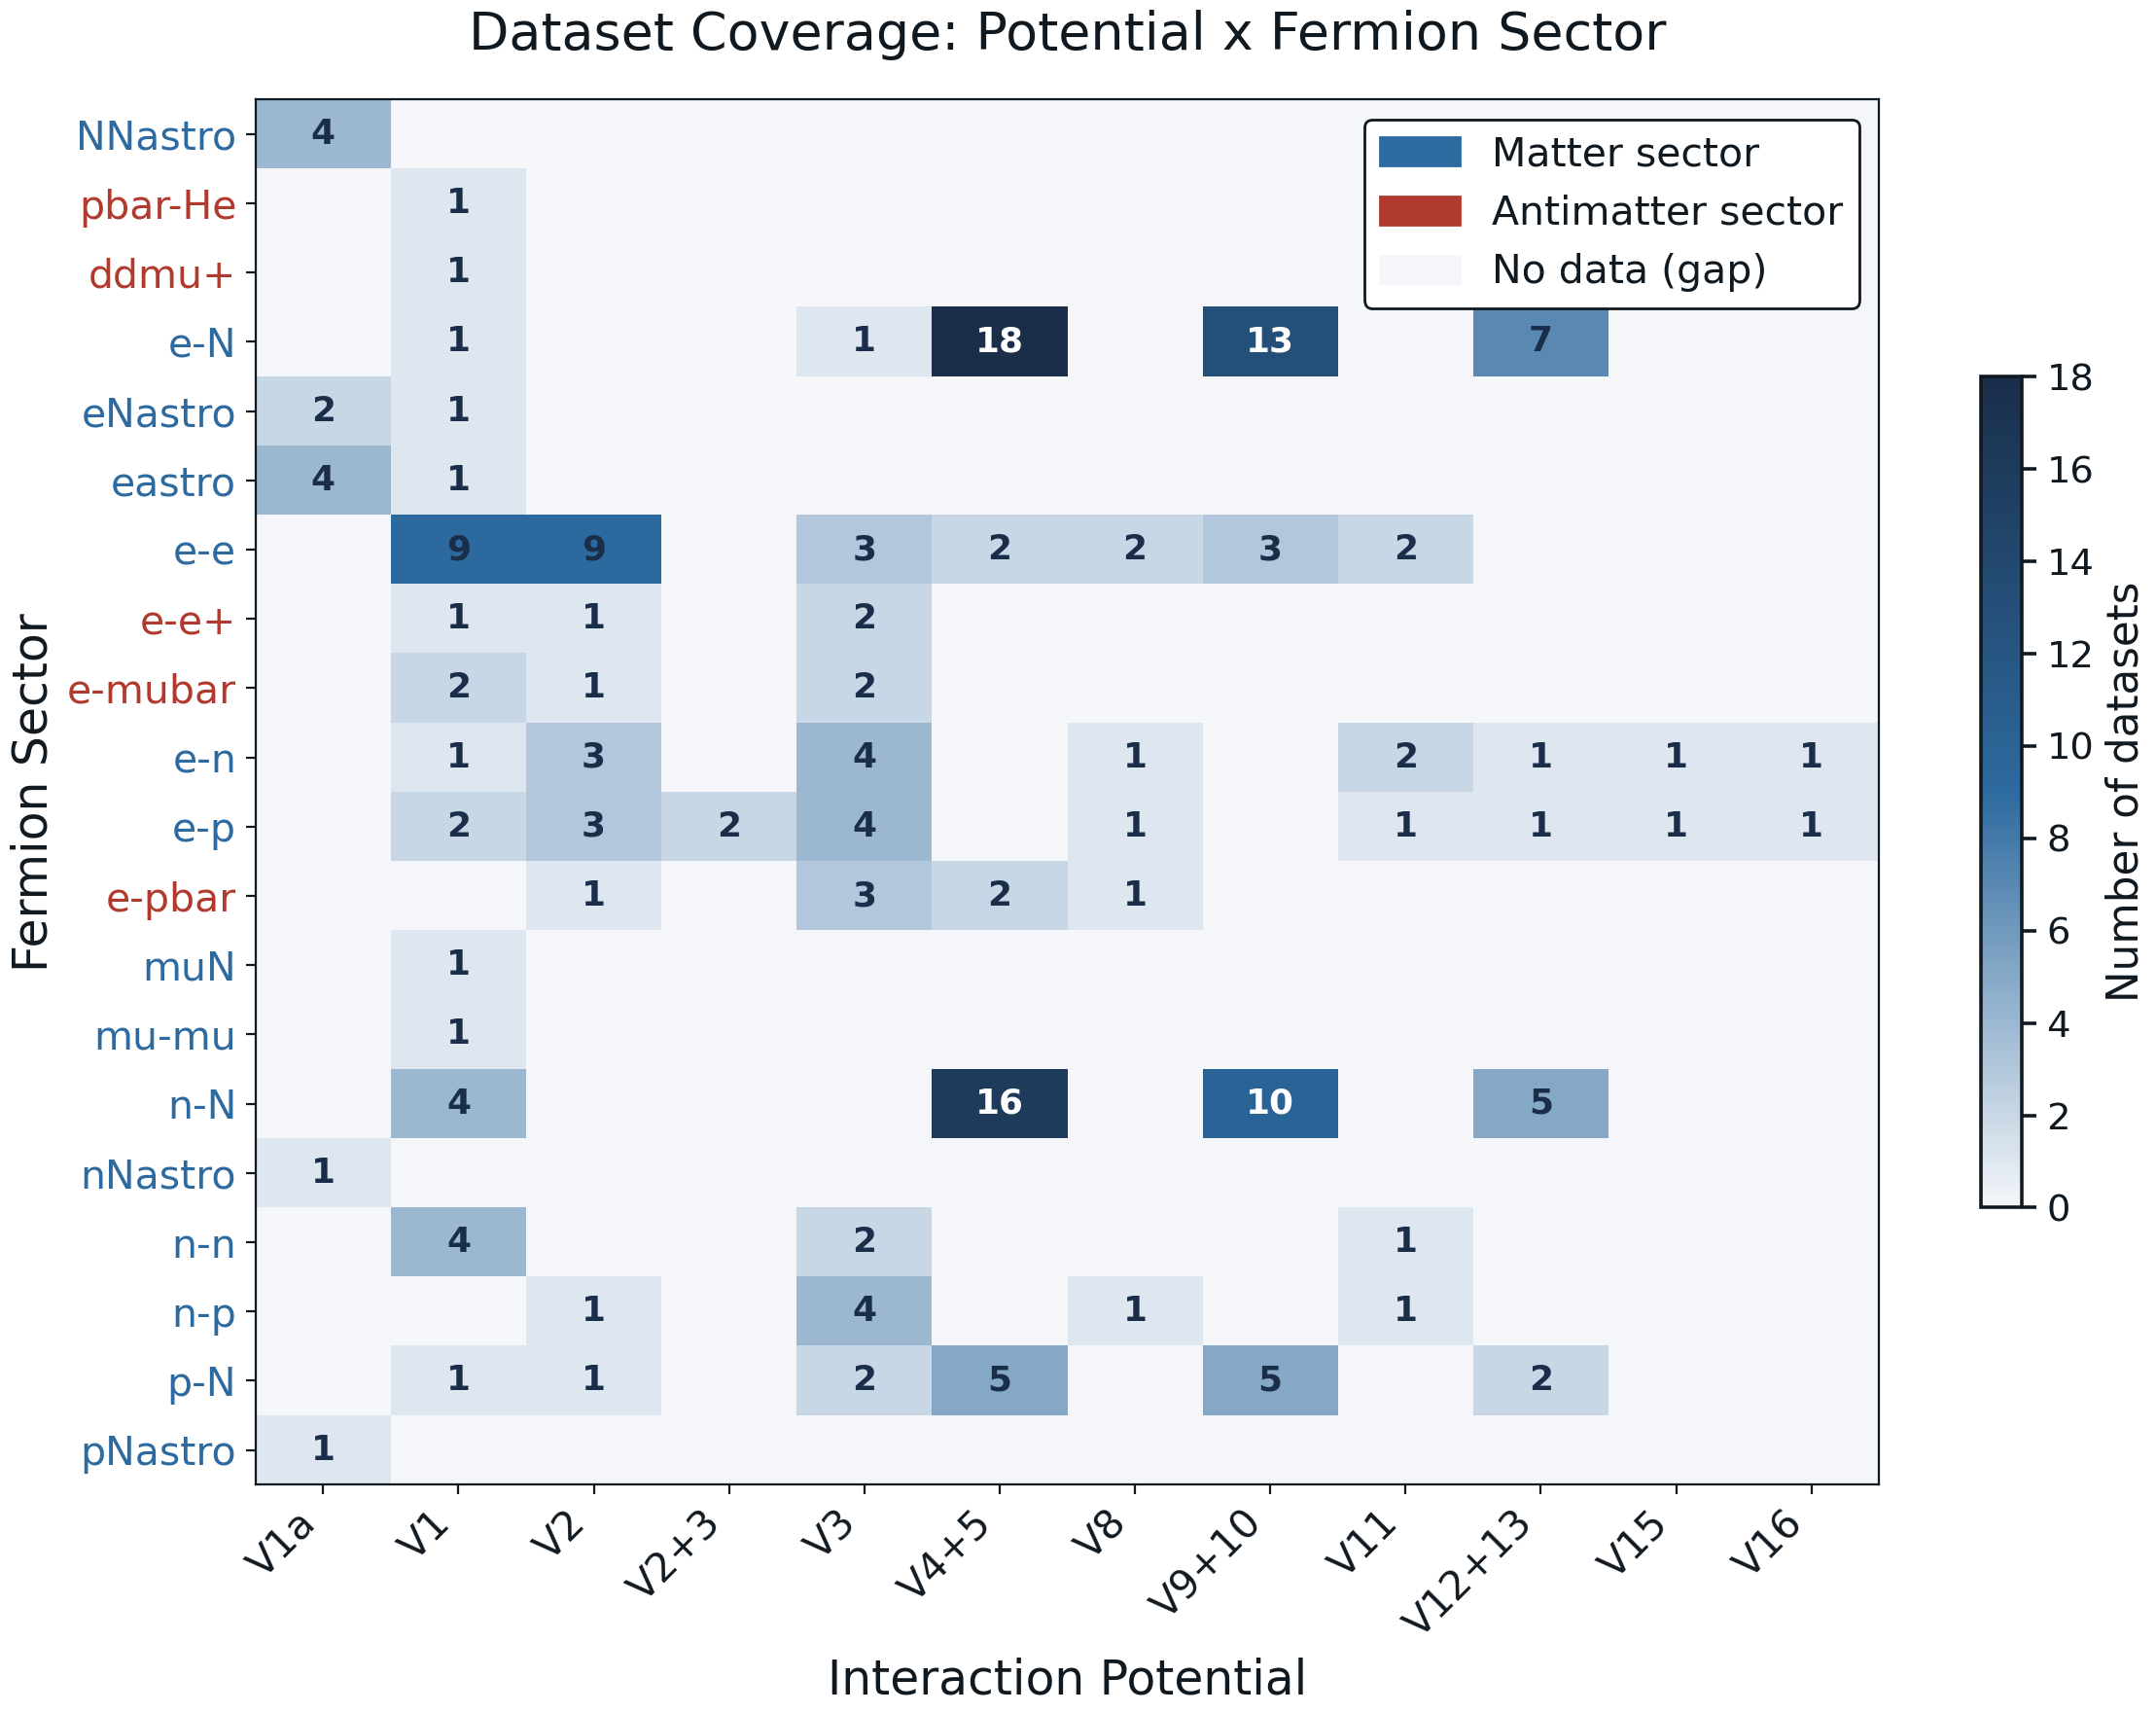
\includegraphics[width=0.78\textwidth]{pair_coverage_matrix.png}
\caption{\label{fig:coverage}%
Dataset coverage by potential and fermion sector; antimatter-sector rows
are highlighted. Cells count independent bounds, not dataset files.}
\end{figure*}

\begin{figure*}[t]
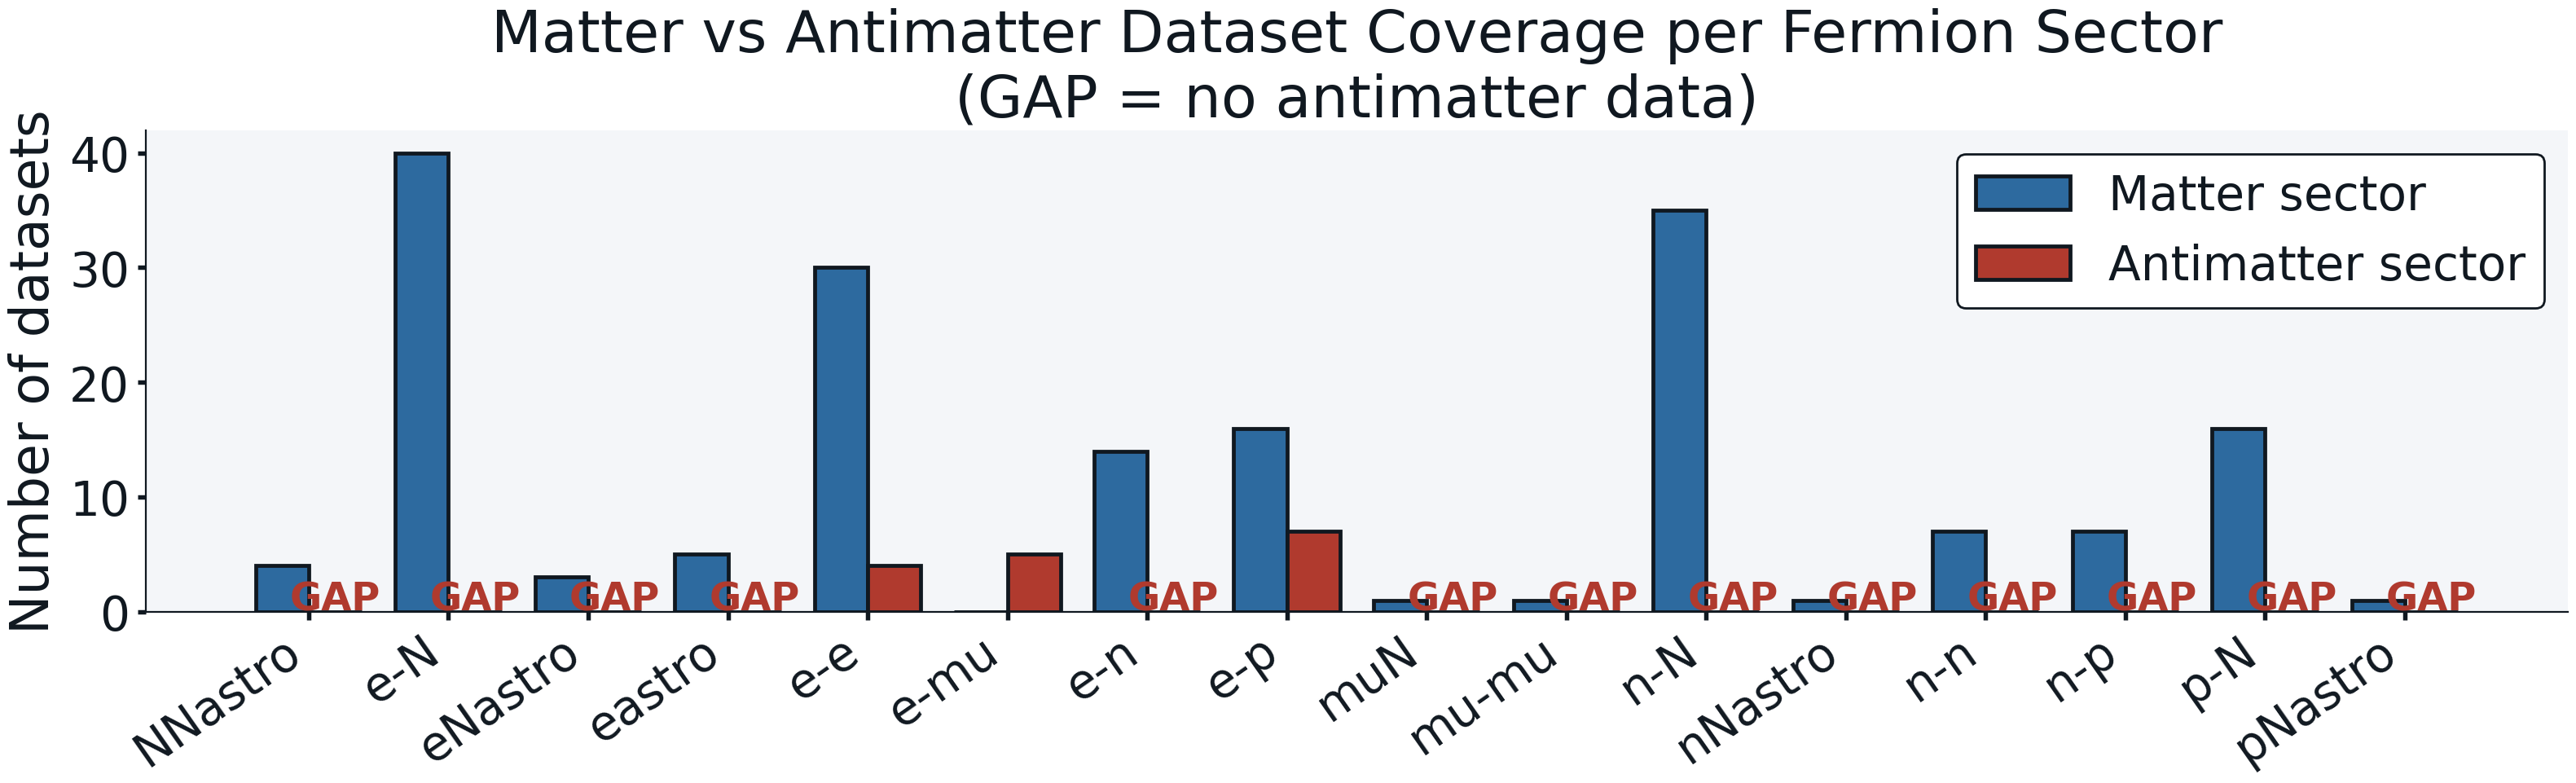
\includegraphics[width=0.95\textwidth]{matter_antimatter_ratio.png}
\caption{\label{fig:ratio}%
Matter versus antimatter dataset coverage per fermion sector. Sectors
marked GAP have no antimatter-sector data at all.}
\end{figure*}

\subsection{Proposed experimental priorities}

Three directions follow. First, antimatter-sector effort is best
prioritized in the $e$-$N$, $n$-$N$, $p$-$N$, $e$-$n$, $n$-$p$ and $n$-$n$
sectors, which together account for 150 of the 225 matter-sector datasets
and zero antimatter-sector ones; precision antiproton experiments such as
BASE \cite{Smorra2017} and antihydrogen spectroscopy such as ALPHA
\cite{Ahmadi2017} are the nearest existing platforms. Second, the same
logic applies at the potential level to $V_{1a}$, $V_{9+10}$ and
$V_{12+13}$, each with 14--31 matter-sector datasets and none on the
antimatter side; $V_1$, $V_2$ and $V_8$ have thin but non-zero coverage
and are better placed as candidates for improving existing precision than
for opening a channel from zero. Third, following the precedent of
Ref.~\cite{Wu2023}, reviewed in Ref.~\cite{Cong2025}, in which
co-magnetometer data taken for sidereal Lorentz- and CPT-violation searches
were reanalyzed as new bounds on the $V_{12+13}$, $V_{4+5}$ and $V_{9+10}$
terms, a systematic reanalysis of existing BASE, ALPHA and
co-magnetometer data is likely to close part of the gap faster, and at
lower cost, than commissioning new measurements.

Across all three, the asymmetry argument of Sec.~\ref{sec:asymmetry}
implies a specific design criterion: a new antimatter-sector bound is
scientifically useful for a CPT test in proportion to how closely it
\emph{matches} the sensitivity of the corresponding matter-sector bound,
not how tight it is in absolute terms. A bound many decades looser than
its matter-sector counterpart will saturate $\Aalpha$ and carry no CPT
information.

% ======================================================================
\section{Limitations}
\label{sec:limitations}

Two limitations of the present database are distinct from the physics
coverage gaps above.

First, the 36 datasets held out of the analysis are excluded rather than
reclassified, and the reasons differ in kind. Twenty-eight are combined envelope curves, twelve in $g_Ag_V$ and
sixteen in $g_pg_s$, that the source compilation marks for review and
assigns no potential; these are not a parsing gap that a naming convention could
close, since no single $V_n$ describes an envelope over several
experiments, and they would have to be decomposed into constituent bounds
before entering a per-potential analysis. Five are the 90\% CL duplicates of the Cong \textit{et al.}\ hydrogen
bounds described in Sec.~\ref{sec:methods}. Two are contributor-template
placeholders that were previously being read as $V_1$ and $V_2$ data on
the strength of a trailing digit in their filenames. The remaining one is
a $g_pg_p$ astrophysical $e$-$N$ bound. It is a real measurement, but its
potential is unassigned upstream, and assigning $V_{1a}$ from the filenames
of related datasets would be a guess, not evidence.

Second, six entries under $V_3$, $V_{9+10}$ and $V_{15}$ report
interaction ranges that are physically implausible, reaching
$\lambda\sim10^{52}$~m against an observable universe of order
$10^{26}$~m, almost certainly from a mis-detected unit token. Three of
the fifteen matched pairs draw on an affected dataset: the $g_Ag_A\cdot
V_3\cdot e$-$e^+$ pair on the matter side, and the two $g_Ag_A\cdot
V_3\cdot e$-$\bar p$ pairs that use the bound of Ref.~\cite{Ficek2018} on
the antimatter side. None of these results is affected, because the
asymmetry is evaluated only on the overlapping range of the two curves and
in every case the implausible tail lies outside it: the ranges used are
$[2.5\times10^{-12},1.6\times10^{-5}]$~m,
$[2.0\times10^{-11},1.0\times10^{-8}]$~m and
$[2.0\times10^{-11},1.3\times10^{-8}]$~m. A broader coverage
claim drawn from the full database without this cleanup would nonetheless
not be reliable.

% ======================================================================
\section{Conclusions}
\label{sec:conclusions}

We have constructed a systematic dictionary between the SME fermion-sector
coefficients $b_\mu$, $d_{\mu\nu}$, $g_{\lambda\mu\nu}$ and $H_{\mu\nu}$
and the Dobrescu--Mocioiu potential basis by explicit Foldy--Wouthuysen
reduction, summarized in Table~\ref{tab:master}. These four are the
complete set generating spin-dependent non-relativistic potentials, so the
dictionary is closed rather than partial: $a_\mu$, $c_{\mu\nu}$ and $e_\mu$
contribute only spin-independent terms and $f_\mu$ none at all through
third order in $1/m$. All four reductions are complete
and agree with established results. The apparent sign discrepancy in the
momentum-linear $d_{ij}$ and $d_{00}$ components against
Ref.~\cite{KosteleckyLane1999} is traced to the momentum-index convention
of that reference, fixed by the free-particle term of the corresponding
derivation \cite{KosteleckyLane1999b}, and is not a feature of the
reduction.

Using this dictionary we defined a CPT asymmetry parameter and evaluated
it against the 247 analyzed constraint datasets. Fifteen
matter--antimatter pairs could be compared, and all show
statistically significant asymmetry after autocorrelation correction. We
showed, however, that this significance cannot be read as evidence of CPT
violation: an asymmetry built from one-sided upper bounds saturates
whenever the two experiments differ in sensitivity, and a spin-independent
scalar channel in our sample shows an asymmetry comparable to the
spin-dependent ones. The practical consequence is a design criterion: what
makes an antimatter-sector bound useful for a CPT test is how well its
sensitivity matches the matter-sector bound, not how tight it is in
absolute terms.

The more important result is what this shows about the data. Only 22 of 247
analyzed datasets involve an antimatter sector; seven of twelve classified
potentials and six of eleven fermion-sector pairs have zero
antimatter-sector coverage despite substantial matter-sector data. The
binding constraint on testing CPT symmetry through exotic spin-dependent
interactions is therefore not matter-sector precision, nor statistical
power, but the near-total absence of comparably precise antimatter-sector
measurements in the very channels where matter-sector data is most
abundant. We offer the mapping table, the compiled database and the
analysis pipeline as an extensible resource for closing that gap, designed
so that future antimatter-sector measurements are incorporated as they are
published.

% ======================================================================
\begin{acknowledgments}
This work was carried out in the Department of Physics, University of
Ibadan. We thank the maintainers of the spin-dependent fifth-force
constraint compilation for making the underlying digitized datasets
publicly available.
\end{acknowledgments}

% ======================================================================
\begin{thebibliography}{99}

\bibitem{Planck2018}
Planck Collaboration (N.~Aghanim \textit{et al.}),
\textit{Planck 2018 results. VI. Cosmological parameters},
Astron. Astrophys. \textbf{641}, A6 (2020).

\bibitem{Colladay1997}
D.~Colladay and V.~A. Kostelecký,
\textit{CPT violation and the standard model},
Phys. Rev. D \textbf{55}, 6760 (1997).

\bibitem{Colladay1998}
D.~Colladay and V.~A. Kostelecký,
\textit{Lorentz-violating extension of the standard model},
Phys. Rev. D \textbf{58}, 116002 (1998).

\bibitem{KosteleckySamuel1989}
V.~A. Kostelecký and S.~Samuel,
\textit{Spontaneous breaking of Lorentz symmetry in string theory},
Phys. Rev. D \textbf{39}, 683 (1989).

\bibitem{KosteleckyLane1999}
V.~A. Kostelecký and C.~D. Lane,
\textit{Constraints on Lorentz violation from clock-comparison
experiments},
Phys. Rev. D \textbf{60}, 116010 (1999).

\bibitem{KosteleckyLane1999b}
V.~A. Kostelecký and C.~D. Lane,
\textit{Nonrelativistic quantum Hamiltonian for Lorentz violation},
J. Math. Phys. \textbf{40}, 6245 (1999).

\bibitem{KosteleckyRussell2011}
V.~A. Kostelecký and N.~Russell,
\textit{Data tables for Lorentz and CPT violation},
Rev. Mod. Phys. \textbf{83}, 11 (2011); living document, updated
annually, 2026 edition, arXiv:0801.0287v19.

\bibitem{Bluhm1999}
R.~Bluhm, V.~A. Kostelecký, and N.~Russell,
\textit{CPT and Lorentz tests in hydrogen and antihydrogen},
Phys. Rev. Lett. \textbf{82}, 2254 (1999).

\bibitem{Dobrescu2006}
B.~A. Dobrescu and I.~Mocioiu,
\textit{Spin-dependent macroscopic forces from new particle exchange},
J. High Energy Phys. \textbf{11}, 005 (2006).

\bibitem{MoodyWilczek1984}
J.~E. Moody and F.~Wilczek,
\textit{New macroscopic forces?},
Phys. Rev. D \textbf{30}, 130 (1984).

\bibitem{Foldy1950}
L.~L. Foldy and S.~A. Wouthuysen,
\textit{On the Dirac theory of spin-1/2 particles and its
non-relativistic limit},
Phys. Rev. \textbf{78}, 29 (1950).

\bibitem{Cong2025}
L.~Cong \textit{et al.},
\textit{Spin-dependent exotic interactions},
Rev. Mod. Phys. \textbf{97}, 025005 (2025).

\bibitem{Cong2025b}
L.~Cong, F.~Ficek, P.~Fadeev, and D.~Budker,
\textit{Improved constraints on exotic electron-proton interactions in
hydrogen},
Phys. Rev. A \textbf{112}, 052824 (2025).

\bibitem{Smorra2017}
C.~Smorra \textit{et al.} (BASE Collaboration),
\textit{A parts-per-billion measurement of the antiproton magnetic
moment},
Nature \textbf{550}, 371 (2017).

\bibitem{Ahmadi2017}
M.~Ahmadi \textit{et al.} (ALPHA Collaboration),
\textit{Observation of the 1S--2S transition in trapped antihydrogen},
Nature \textbf{541}, 506 (2017).

\bibitem{Adkins2022}
G.~S. Adkins, D.~B. Cassidy, and J.~Pérez-Ríos,
\textit{Precision spectroscopy of positronium: Testing bound-state QED
theory and the search for physics beyond the Standard Model},
Phys. Rep. \textbf{975}, 1 (2022).

\bibitem{Alighanbari2020}
S.~Alighanbari, G.~S. Giri, F.~L. Constantin, V.~I. Korobov, and
S.~Schiller,
\textit{Precise test of quantum electrodynamics and determination of
fundamental constants with HD$^+$ ions},
Nature \textbf{581}, 152 (2020).

\bibitem{Bordag2001}
M.~Bordag, U.~Mohideen, and V.~M. Mostepanenko,
\textit{New developments in the Casimir effect},
Phys. Rep. \textbf{353}, 1 (2001).

\bibitem{Chen2016}
Y.-J. Chen, W.~K. Tham, D.~E. Krause, D.~López, E.~Fischbach, and
R.~S. Decca,
\textit{Stronger limits on hypothetical Yukawa interactions in the
30--8000 nm range},
Phys. Rev. Lett. \textbf{116}, 221102 (2016).

\bibitem{Delaunay2017}
C.~Delaunay, C.~Frugiuele, E.~Fuchs, and Y.~Soreq,
\textit{Probing new spin-independent interactions through precision
spectroscopy in atoms with few electrons},
Phys. Rev. D \textbf{96}, 115002 (2017).

\bibitem{Fadeev2019}
P.~Fadeev, Y.~V. Stadnik, F.~Ficek, M.~G. Kozlov, V.~V. Flambaum, and
D.~Budker,
\textit{Revisiting spin-dependent forces mediated by new bosons:
Potentials in the coordinate-space representation for macroscopic- and
atomic-scale experiments},
Phys. Rev. A \textbf{99}, 022113 (2019).

\bibitem{Fadeev2022}
P.~Fadeev, F.~Ficek, M.~G. Kozlov, D.~Budker, and V.~V. Flambaum,
\textit{Pseudovector and pseudoscalar spin-dependent interactions in
atoms},
Phys. Rev. A \textbf{105}, 022812 (2022).

\bibitem{Ficek2017}
F.~Ficek, D.~F. Jackson Kimball, M.~G. Kozlov, N.~Leefer, S.~Pustelny,
and D.~Budker,
\textit{Constraints on exotic spin-dependent interactions between
electrons from helium fine-structure spectroscopy},
Phys. Rev. A \textbf{95}, 032505 (2017).

\bibitem{Ficek2018}
F.~Ficek, P.~Fadeev, V.~V. Flambaum, D.~F. Jackson Kimball, M.~G. Kozlov,
Y.~V. Stadnik, and D.~Budker,
\textit{Constraints on exotic spin-dependent interactions between matter
and antimatter from antiprotonic helium spectroscopy},
Phys. Rev. Lett. \textbf{120}, 183002 (2018).

\bibitem{Heckel2008}
B.~R. Heckel, E.~G. Adelberger, C.~E. Cramer, T.~S. Cook,
S.~Schlamminger, and U.~Schmidt,
\textit{Preferred-frame and CP-violation tests with polarized electrons},
Phys. Rev. D \textbf{78}, 092006 (2008).

\bibitem{Hoskins1985}
J.~K. Hoskins, R.~D. Newman, R.~Spero, and J.~Schultz,
\textit{Experimental tests of the gravitational inverse-square law for
mass separations from 2 to 105 cm},
Phys. Rev. D \textbf{32}, 3084 (1985).

\bibitem{Jiao2020}
M.~Jiao, X.~Rong, H.~Liang, Y.-F. Cai, and J.~Du,
\textit{Searching for an exotic spin-dependent interaction between
electrons at the nanometer scale with molecular rulers},
Phys. Rev. D \textbf{101}, 115011 (2020).

\bibitem{Kapner2007}
D.~J. Kapner, T.~S. Cook, E.~G. Adelberger, J.~H. Gundlach,
B.~R. Heckel, C.~D. Hoyle, and H.~E. Swanson,
\textit{Tests of the gravitational inverse-square law below the
dark-energy length scale},
Phys. Rev. Lett. \textbf{98}, 021101 (2007).

\bibitem{Karshenboim2011}
S.~G. Karshenboim,
\textit{Hyperfine structure interval of the 2s state of hydrogenlike
atoms and a constraint on a pseudovector boson with mass below 1 keV},
Phys. Rev. A \textbf{83}, 062119 (2011).

\bibitem{Lee2020}
J.~G. Lee, E.~G. Adelberger, T.~S. Cook, S.~M. Fleischer, and
B.~R. Heckel,
\textit{New test of the gravitational $1/r^2$ law at separations down to
52 $\mu$m},
Phys. Rev. Lett. \textbf{124}, 101101 (2020).

\bibitem{Rong2018a}
X.~Rong \textit{et al.},
\textit{Constraints on a spin-dependent exotic interaction between
electrons with single electron spin quantum sensors},
Phys. Rev. Lett. \textbf{121}, 080402 (2018).

\bibitem{Rong2018b}
X.~Rong \textit{et al.},
\textit{Searching for an exotic spin-dependent interaction with a single
electron-spin quantum sensor},
Nat. Commun. \textbf{9}, 739 (2018).

\bibitem{Salumbides2014}
E.~J. Salumbides, W.~Ubachs, and V.~I. Korobov,
\textit{Bounds on fifth forces at the sub-\AA{} length scale},
J. Mol. Spectrosc. \textbf{300}, 65 (2014).

\bibitem{Tan2020}
W.-H. Tan \textit{et al.},
\textit{Improvement for testing the gravitational inverse-square law at
the submillimeter range},
Phys. Rev. Lett. \textbf{124}, 051301 (2020).

\bibitem{Vasilakis2009}
G.~Vasilakis, J.~M. Brown, T.~W. Kornack, and M.~V. Romalis,
\textit{Limits on new long range nuclear spin-dependent forces set with a
K--$^3$He co-magnetometer},
Phys. Rev. Lett. \textbf{103}, 261801 (2009).

\bibitem{Wu2023}
L.~Y. Wu, K.~Y. Zhang, M.~Peng, J.~Gong, and H.~Yan,
\textit{New limits on exotic spin-dependent interactions at astronomical
distances},
Phys. Rev. Lett. \textbf{131}, 091002 (2023).

\end{thebibliography}

\end{document}
